% !TEX program = xelatex
% ============================================================================
%  M2-Alpha Technical Report (English version)
%  Build: xelatex M2Alpha_Technical_Report_EN.tex (run twice for references)
%  English translation of M2Alpha_Technical_Report.tex.
%  Changes vs. the Chinese original: ctexart -> article; ctex/CJK font setup,
%  \newCJKfontfamily, and \ctexset removed; \heiti redefined as a no-op so the
%  custom commands (\comp, \note, ...) keep working without fandol.
% ============================================================================
\documentclass[a4paper,11pt]{article}

% ---------- Layout ----------
\usepackage[top=2.5cm,bottom=2.5cm,left=2.6cm,right=2.6cm]{geometry}
\linespread{1.2}
\setlength{\parskip}{0.35em}

% ---------- Math ----------
\usepackage{amsmath,amssymb,amsfonts,bm,mathtools}

% ---------- Figures / Tables ----------
\usepackage{graphicx}
\usepackage{float}
\usepackage{booktabs}                       % \toprule \midrule \bottomrule
\usepackage{array,multirow,makecell}
\usepackage{tabularx}
\usepackage{caption}
\usepackage{subcaption}
\usepackage{xcolor}
\usepackage{fontawesome5}

% ---------- CJK support (so Chinese stock names can be kept in their original form) ----------
% Uses macOS Songti SC. On Linux/Windows replace with any installed CJK serif
% (e.g. Noto Serif CJK SC, or FandolSong under TeX Live with fandol registered).
\usepackage{xeCJK}
\setCJKmainfont{Songti SC}

% ---------- Lists / Links ----------
\usepackage{enumitem}
\setlist{nosep,leftmargin=2em,topsep=0.3em}
\usepackage[colorlinks=true,linkcolor=black,citecolor=blue!55!black,urlcolor=blue!55!black]{hyperref}

% ---------- Section title styling (replaces ctex \ctexset) ----------
\usepackage{titlesec}
\titleformat{\section}{\Large\bfseries}{\thesection}{0.8em}{}
\titleformat{\subsection}{\large\bfseries}{\thesubsection}{0.7em}{}
\titleformat{\subsubsection}{\normalsize\bfseries}{\thesubsubsection}{0.6em}{}
\titleformat{\paragraph}[runin]{\normalsize\bfseries}{\theparagraph}{0.6em}{}

% Captions: small, bold label
\captionsetup{font=small,labelfont=bf,labelsep=quad}
\captionsetup[table]{skip=4pt}

% ---------- Custom commands (same semantics as the Chinese original) ----------
\newcommand{\msq}{\texorpdfstring{M\textsuperscript{2}}{M2}}             % M² Block
\newcommand{\msqa}{\texorpdfstring{M\textsuperscript{2}-Alpha}{M2-Alpha}} % M²-Alpha
\newcommand{\note}[1]{\textcolor{blue!55!black}{\small[Note: #1]}}      % inline note
\newcommand{\bestckpt}{\textsuperscript{\dag}}                          % best-ckpt marker
\newcommand{\msd}[2]{$#1{\scriptstyle\pm#2}$}                           % mean±std
% Bold run-in heading for sub-components inside a section (RSR-style)
\newcommand{\comp}[1]{\par\smallskip\noindent\textbf{#1.}\ }
% \heiti is a ctex command; keep it as a no-op so leftover uses do not break.
\providecommand{\heiti}{}

% ============================================================================
\title{\bfseries \msqa: Thinking Like a Trader via Iterative\\
       Dual-Axis Attention for Stock Ranking\\[4pt]\large Technical Report}
\author{M2-Alpha Project\\[3pt]
{\normalsize\faGithub~\href{https://github.com/Johnny-xuan/M2-Alpha}{github.com/Johnny-xuan/M2-Alpha}}}
\date{\today}

\begin{document}
\maketitle

% ---------------------------------------------------------------- Abstract
\begin{abstract}
\noindent
A-share cross-sectional stock selection---ranking the universe every day and
buying a basket of the top names---is a low-SNR task: individual signals are
buried in noise and market regimes switch frequently. An experienced trader
reads the tape along two axes simultaneously: along the \emph{time axis} to
follow a stock's own trajectory, and along the \emph{cross-sectional axis} to
compare it against the whole market, iterating between the two views until the
ranking is settled. We build on this intuition and propose a dual-axis
Transformer, \msqa{}, with two core designs. \textbf{First}, the dual-axis
interaction is packaged as a stackable feature primitive, the \msq{} Block
(Micro axis: causal temporal attention reads a single stock's trajectory; Macro
axis: cross-sectional attention performs the cross-sectional comparison); stacking $L$
layers lets the two axes iteratively re-read and refine each other.
\textbf{Second}, we keep the full $(S,T,D)$ representation throughout---never
flattening the time axis at the end---and apply dense cross-sectional ranking
supervision at every time step in the window. A controlled ablation with a
fixed architecture that changes only the supervision density confirms its
contribution: dense supervision significantly outperforms last-step-only
supervision under both the ``validation-selected checkpoint'' and the
``best-checkpoint'' protocols (error bars do not overlap).

Under the best-checkpoint protocol, \msqa{} reaches a cumulative $+155\%$ on
the 2025--26 test period, ahead of 13 representative baselines; but we also
report a deployable validation-selected figure ($+56\pm60\%$) and document a
counter-intuitive finding: validation IC is \emph{negatively} correlated with
out-of-sample return ($-0.75$), and the same configuration swings by $\pm 60$
percentage points solely due to seed and checkpoint choice---larger than the
effect of most architectural changes. Building on this, we propose a unified
evaluation protocol (best ckpt for the capability ceiling, multi-seed
mean$\pm$std, a $\pm 60$pp variance redline) and re-examine architectural
choices under it: both axes are indispensable (removing either costs about
$45$pp), while the marginal gains of stacking depth and of alternative training
objectives mostly fall inside the noise band. The interpretability analysis
further offers the \emph{most self-consistent mechanistic explanation} of Macro
given the current evidence: it behaves like a learned cross-sectional
denoiser---pulling each stock's prediction toward the consensus of a
data-driven set of correlated peers and suppressing stock-specific noise (this
peer set barely overlaps with Shenwan industries, normalized mutual information
NMI only $0.23$, so it is not simple industry demeaning). In a market where
signals are drowned by noise, denoising is the most plausible reason it works
(we provide multiple lines of suggestive evidence, but no direct causal proof
of variance reduction).

The point of this paper is not the $+155\%$ number; it is the few conclusions
that survive the across-seed variance ($\pm 60$pp), and a judgment: under low
SNR, \emph{how} you train and select checkpoints matters more for the final
return than \emph{which} architecture you use. Holding the model's signal fixed
and changing only the trading strategy (e.g.\ position concentration) can move
the return by $130$ percentage points---the same order as architectural changes,
which is direct circumstantial evidence for this judgment.

\medskip
\noindent\textbf{Keywords:} cross-sectional stock selection; dual-axis
Transformer; cross-sectional attention; learning-to-rank; interpretability;
variance control
\end{abstract}

% ================================================================ 1 Introduction
\section{Introduction}\label{sec:intro}

The core goal of quantitative stock selection is not to predict the exact
tomorrow's return of a single stock, but to pick, each day, a small set of the
most worth-buying names from thousands of candidates. This is essentially a
\emph{cross-sectional ranking} problem, and one of the most representative
applications of deep learning in quantitative investment~\cite{survey}. The
task is especially hard in the A-share market, and the difficulty comes from
noise---which has two layers. One is universal: short-horizon cross-sectional
returns have very low predictability to begin with, and even a good model only
achieves validation IC on the order of $0.02$; the signal is inherently weak.
The other is an A-share-specific amplifier: retail dominance and high turnover
mean prices are pushed around by sentiment and order flow, diluting
fundamental signals; policy and theme-driven moves make cross-sectional
returns highly contingent on concept rotation and exogenous shocks (later we
will even see stocks renaming themselves to chase the quantum concept); fast
style switching and rapid factor decay mean a signal that works this month may
fail next month; and price limits ($\pm10\%$) plus T+1 settlement truncate and
distort next-day returns. Together, these make ``today's pattern will still
hold tomorrow'' a faint hope---this is the root cause of both the $\pm 60$pp
seed variance and the negative IC--return relation (\S\ref{sec:select}), and it
is also the premise for why a denoising mechanism like Macro is needed.

Yet an experienced trader, when making a buy/sell decision, is in fact doing
two things at once (Fig.~\ref{fig:trader}): reading a stock's own trajectory
and pattern along the \emph{time axis}, while comparing it with the whole
market along the \emph{cross-sectional axis} to judge whether it is strong or
weak right now. The two views are not sequential---they alternate and
corroborate each other until the trader is confident enough to commit to a
buy list. The entire intuition behind our method comes from this process.

\begin{figure}[t]
\centering
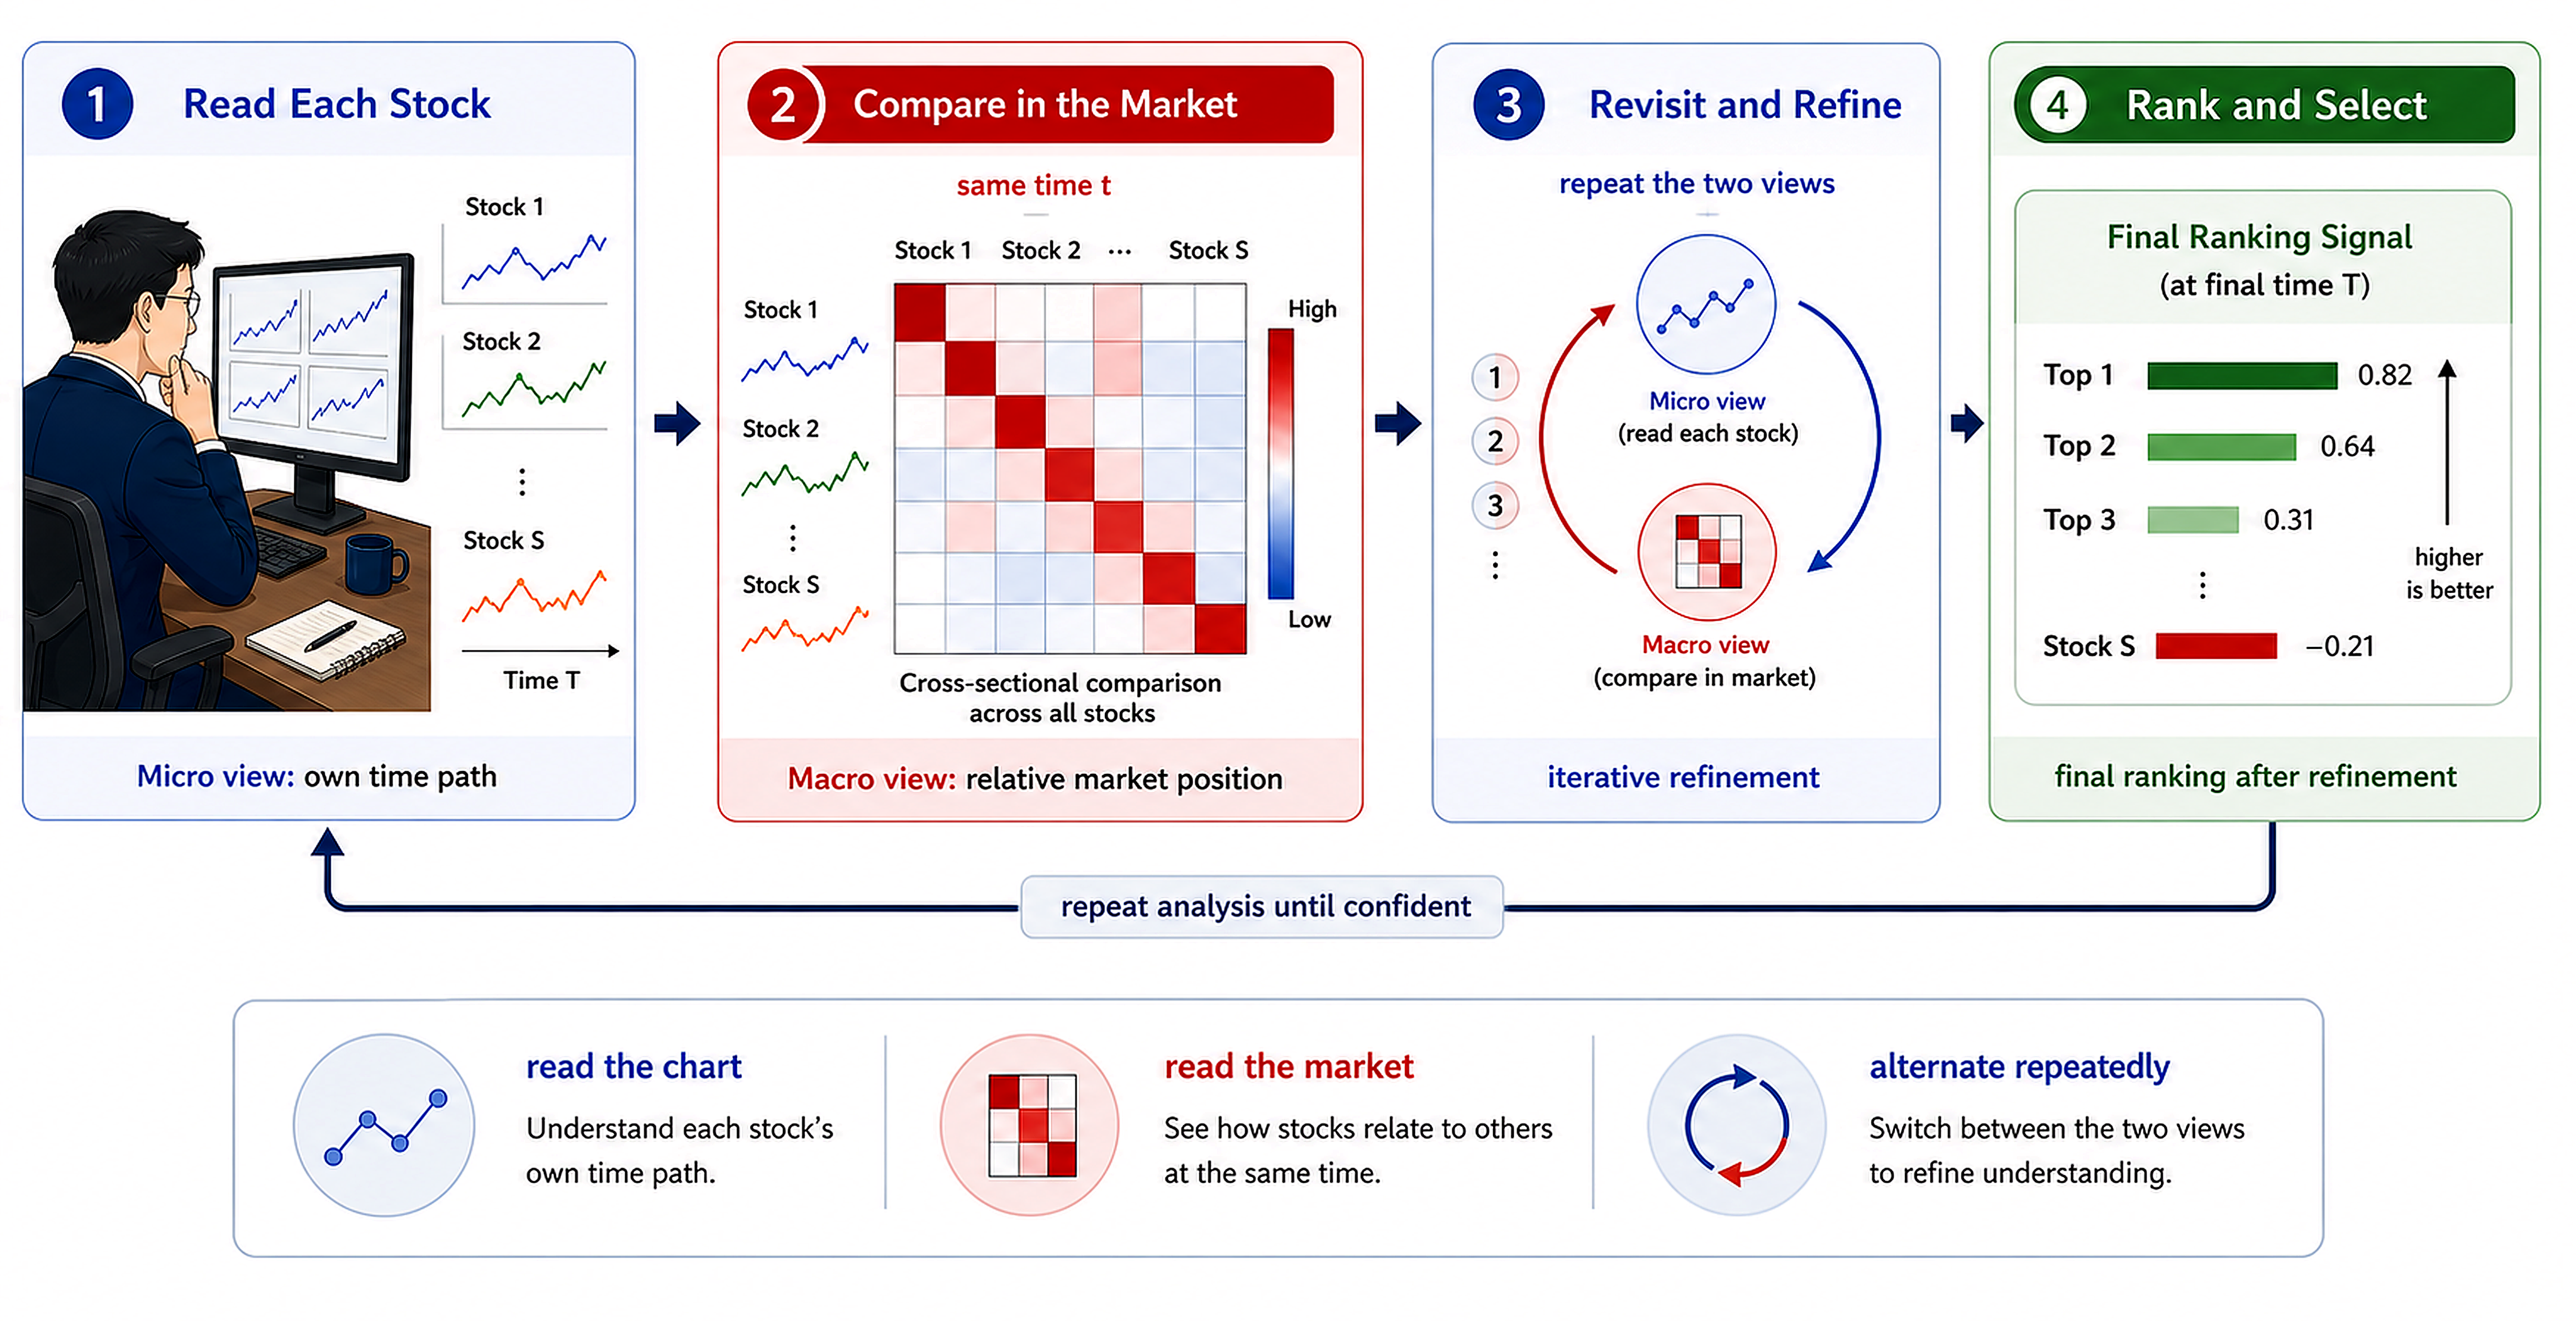
\includegraphics[width=\linewidth]{figures/fig_trader.png}
\caption{The trader's dual-view cognition: reading a single stock's trajectory
along the time axis (the Micro view) and comparing it across the market along
the cross-sectional axis (the Macro view), iterating between the two views
until a final ranking is produced. We explicitly model this process as a
stackable \msq{} Block.}
\label{fig:trader}
\end{figure}

Deep learning for stock selection has evolved from early models that build only
per-stock time series (RNN, CNN) to dual-axis architectures that model both the
time and cross-sectional dimensions jointly. Existing dual-axis methods,
however, broadly share two shortcomings. First, \textbf{the two views are
applied only once}: look at the own-trend first, then the cross-sectional
position, output the result, done. But the two signals are \emph{interdependent}:
reading a temporal pattern depends on the cross-sectional context (the same
``$-5\%$ drop'' means opposite things in a bull market versus a crash), and
judging the cross-sectional position depends on the temporal trajectory
(``high today'' may be a sustained climb or a just-peaked spike); in a single
pass, both views compute without knowing the other's conclusion, leaving no
room for mutual correction. Second, \textbf{the time dimension is flattened
too early}: many methods compress the entire lookback window into a single
vector at the end before predicting, discarding per-day states within the
window, even though short-term momentum is one of the most stable signals in
A-shares.

Building on these observations, our central claim is that to unlock this
mutual dependence the two views must be \textbf{explicitly decoupled} and then
\textbf{iteratively refined against each other}, rather than being run once in
sequence. We thus propose \msqa{} (Micro--Macro Alpha Engine): the micro
attention along the time axis (Micro) and the macro attention along the
cross-sectional axis (Macro) are packaged into a stackable \msq{} Block, and
stacking multiple layers lets the two views recursively deepen each other
(corresponding to the repeated re-reading in the third panel of
Fig.~\ref{fig:trader}). The remaining design choices---keeping the $(S,T,D)$
representation throughout, applying dense supervision at every time step, and
\emph{not} injecting market state explicitly---are developed in
\S\ref{sec:method}.

In addition, low SNR brings a counter-intuitive phenomenon that runs through
the whole paper: \emph{more accurate prediction does not imply more profitable
selection}. For example, within a single training run, the checkpoint selected
by ``highest validation IC'' (ep34) achieves only $+67.2\%$ out of sample,
while ep13---whose validation IC is only mid-range---reaches the highest
$+170.9\%$; validation IC and out-of-sample return systematically diverge. This
phenomenon and its implications for model selection criteria are detailed in
\S\ref{sec:select}.

\noindent\textbf{Two core design innovations.}
\begin{itemize}
  \item \textbf{(Dual-axis modularization and iterative re-reading)} We package
        the dual-axis interaction into a stackable, per-axis-disableable feature
        primitive, the \msq{} Block, and let Micro and Macro recursively refine
        each other through stacking. We do not claim to invent the idea of
        dual-axis modeling (it has a clear lineage, see \S\ref{sec:rw-dual});
        rather, we organize it into a \emph{dissectable, iterable} unit. This
        contribution is supported by the dual-axis ablation, the stacking-depth
        sweep, and the equal-parameter widening control (\S\ref{sec:pillars},
        \ref{sec:depth}).
  \item \textbf{(Keeping $(S,T,D)$ and dense temporal supervision)} We keep the
        stock$\times$time$\times$hidden three-dimensional representation
        throughout---never flattening the time axis at the end---and apply
        dense cross-sectional ranking supervision at every time step in the
        window. \emph{Keeping the time dimension} (a representation choice) and
        \emph{dense supervision} (an objective choice) are two separable
        decisions; we use a controlled ablation with a fixed architecture that
        only changes the loss from the full window to last-step-only, isolating
        and \emph{confirming} the contribution of dense supervision
        itself---under both protocols it significantly outperforms last-step-only
        supervision with non-overlapping error bands (\S\ref{sec:abl-dense}).
\end{itemize}

\noindent\textbf{Experiments and methodological contributions.}
\begin{itemize}
  \item \textbf{(Evaluation protocol and the checkpoint-selection failure)} We
        propose a unified evaluation protocol (best checkpoint + multi-seed +
        a $\pm 60$pp variance redline) and obtain a transferable finding: under
        low SNR, validation IC is \emph{inversely} related to out-of-sample
        return, so the standard best-valid-IC selection rule systematically
        picks worse-generalizing models (\S\ref{sec:select}).
  \item \textbf{(Macro as a learned cross-sectional denoiser---an empirical
        finding)} Attention analysis, the weighted-shrinkage sweep, and the
        whole-market co-movement test jointly show that, after training, Macro
        behaves like an \emph{adaptive cross-sectional denoiser}, pulling each
        stock's prediction toward the consensus of a data-driven set of
        correlated peers and suppressing stock-specific noise. Its soft
        grouping has only $0.23$ NMI with Shenwan industries, so it references
        \emph{neither} industry means \emph{nor} external relation graphs
        (\S\ref{sec:macro}). This is a \emph{post-hoc} explanation for a module
        designed for cross-sectional reference, not a design innovation declared
        in advance, and it admits a natural interpretation under the
        James--Stein / empirical-Bayes shrinkage framework.
  \item \textbf{(Empirics and honest attribution)} Against CSI300 and 13
        representative methods, \msqa{} leads in return under the best-checkpoint
        protocol (seed42 $+170.9\%$, multi-seed $+155\%$, higher than all
        reproduced baselines, e.g.\ RSR $+94.5\%$, adversarial ALSTM $+78.9\%$).
        But the paper's output is not just the return; it is also the few robust
        conclusions that survive the variance redline, and the judgment that,
        under low SNR, how you train and select checkpoints matters more than the
        architecture itself.
\end{itemize}

\noindent\textbf{Organization.}
\S\ref{sec:related} reviews related work; \S\ref{sec:data} covers data, task,
and the feature-engineering pipeline; \S\ref{sec:method} details the
architecture and training of \msqa{}; \S\ref{sec:exp} reports the experimental
setup, the unified evaluation protocol, the main comparison, the ablation
evidence for the two innovations, and the mechanism of Macro; \S\ref{sec:discuss}
discusses limitations; \S\ref{sec:conclusion} concludes.

% ================================================================ 2 Related Work
\section{Related Work and Preliminaries}\label{sec:related}

\subsection{Single-stock temporal modeling}\label{sec:rw-seq}
The earliest family of methods treats each stock as an independent time series.
Recurrent networks (LSTM~\cite{lstm}, GRU) and their attention-augmented
variants (ALSTM~\cite{alstm}) model per-stock history along the time axis to
predict future return or up/down move; the frequency-domain method
SFM~\cite{sfm} decomposes hidden states into different frequency components to
capture multi-period patterns; convolutional methods use 1-D convolution along
the time axis to extract local patterns. These three use recurrence,
convolution, and attention respectively as the inductive bias for temporal
modeling, but share a stronger assumption---\emph{single-stock, purely
temporal}: a stock's future is determined mainly by its own history. For a
selection task whose goal is \emph{relative ranking}, this assumption discards
cross-sectional information, while ``how other stocks performed on the same
day'' is exactly the reference frame that defines ``whether this stock is
strong.''

\subsection{Dual-axis dependency modeling: graph priors vs.\ data-driven}\label{sec:rw-dual}
To bring in cross-sectional information, one line of work models both the time
axis and the stock axis jointly. By ``where inter-stock relations come from,''
it splits into two branches.

\textbf{Graph priors.} This branch explicitly supplies a stock relation
graph. RSR~\cite{rsr} builds an adjacency matrix from industries, supply
chains, and similar relations and smooths related stocks' representations via a
Temporal Graph Convolution; HIST~\cite{hist} further distinguishes predefined
concepts from concepts mined out of data. Their relations are \emph{exogenous},
depend on the coverage and timeliness of the relation data, and the relation
graph is usually static.

\textbf{Data-driven.} This branch does not prescribe relations; instead,
it lets attention learn the mutual influence between stocks along the stock
axis. DTML~\cite{dtml} feeds both market state and per-stock representations
into its so-called data-axis Transformer (i.e.\ the stock axis), letting stocks
attend to each other; MASTER~\cite{master} alternates attention on the time axis
and the stock axis and uses market state to modulate per-stock features.
Related efforts include StockMixer~\cite{stockmixer} (which uses MLP-mixing to
alternately mix the time, feature, and stock dimensions) and the general
multivariate time-series model Crossformer~\cite{crossformer} (whose
Two-Stage Attention attends along the time and variable dimensions separately).

This paper follows the data-driven line, with MASTER as the most direct point
of comparison. The idea of \emph{dual-axis dependency modeling} was established
jointly by the works above; we do not claim first authorship. The key
difference from MASTER is in how the dual axis is handled: MASTER runs a
\emph{single} pass (time axis once, stock axis once, then flattens the time
dimension for prediction), whereas we organize the dual-axis interaction into a
\emph{stackable, per-axis-disableable} unit, keep the $(S,T,D)$ representation
throughout, use causal temporal attention, and apply dense cross-sectional
ranking supervision at every time step.

\subsection{Supervision and temporal compression}\label{sec:rw-sup}
Our second design choice concerns \emph{how to treat the time window}; we give
its literature background separately here. Many temporal stock-selection models
\emph{compress the whole lookback window into a single end vector} before
prediction: recurrent networks take the last hidden state $h_T$; attention
models (such as MASTER) pool the time dimension after the stock-axis
interaction or keep only the last step---and then predict only on this
compressed representation, with only the last-step state under supervision.
This conflates two \emph{separable} design decisions: one is
\textbf{representation design}---whether to flatten the time dimension or keep
the full $(S,T,D)$; the other is \textbf{objective design}---whether to
supervise only the last step or to densely supervise every time step in the
window. The former concerns whether temporal and cross-sectional information
can interleave fully at every layer; the latter concerns gradient density
during training.

Our second innovation sits exactly on this pair of choices: \emph{keep the
$(S,T,D)$ representation} (do not flatten the time dimension mid-network) and
\emph{apply dense supervision to all time steps}. Since the two are usually
adopted together and hard to attribute, we separate them in the
experiments---fixing the architecture and changing only the loss from
``full-window supervision'' to ``last-step-only'' to isolate the contribution of
dense supervision itself (\S\ref{sec:abl-dense}). This decomposition
perspective is the main positional difference between us and the compressive
approaches above.

\subsection{Training paradigms}\label{sec:rw-train}
Beyond architecture, training objectives and regularization are equally
important under low SNR. AdvALSTM~\cite{advalstm} adds adversarial perturbations
to the input or hidden layers to improve generalization; TRA~\cite{tra} sets up
multiple ``trading patterns'' and uses optimal transport to route samples to
different patterns, mitigating overfitting to a single pattern; RSR~\cite{rsr}
directly optimizes a pairwise ranking loss rather than per-stock regression.
These training paradigms designed specifically for low SNR show higher task-fit
in the failure diagnosis of \S\ref{sec:main}---how well a paradigm matches the
task is often more decisive for the final outcome than how elaborate the
architecture is.

\paragraph{Inductive bias and dual-axis handling}
Seen from a higher level, the methods above can be characterized along two
dimensions (Table~\ref{tab:cnn-track}): the inductive bias for temporal modeling
(recurrent / convolutional / attention); and how the time axis and stock axis
are handled---\emph{fused} in a single forward pass, or \emph{decoupled} and
woven together iteratively. The overwhelming majority of prior methods belong
to the former; our entry point is the latter: decouple the two axes and refine
iteratively.

\begin{table}[H]
\centering
\caption{Temporal inductive bias $\times$ dual-axis handling. Most methods fuse
the two axes in a single forward pass; we decouple them and iterate.}
\label{tab:cnn-track}
\begin{tabularx}{\linewidth}{l>{\raggedright\arraybackslash}X>{\raggedright\arraybackslash}X}
\toprule
Temporal inductive bias & Representative methods & Dual-axis handling \\
\midrule
Recurrent (RNN)    & ALSTM, DTML            & Single-pass fuse \\
Conv/Mix (CNN/MLP) & Temporal conv, StockMixer & Single-pass fuse \\
Attention          & MASTER; \msqa{} (ours) & MASTER single-pass fuse; \textbf{ours: decouple + iterate} \\
\bottomrule
\end{tabularx}
\end{table}

\paragraph{Notation conventions}
We use bold capitals for matrices / tensors (e.g.\ $\bm{X}$), bold lowercase for
vectors (e.g.\ $\bm{x}$), and plain lowercase for scalars. The number of stocks
is $S$, time steps $T$, input feature dimension $F$, hidden dimension $D$. The
full notation is in Table~\ref{tab:notation}.

% ================================================================ 3 Data, Task, Feature Engineering
\section{Data, Task, and Feature Engineering}\label{sec:data}
In quantitative tasks the data-processing pipeline is the foundation of
credibility: it directly determines whether there is future-information
leakage, whether labels are aligned, whether features are tradable, and whether
the backtest is trustworthy. This section first formalizes the task, then lays
out the full data flow from raw quotes to the feature tensor
$\bm{X}\in\mathbb{R}^{S\times T\times F}$ and from future returns to the labels
$\bm{Y}\in\mathbb{R}^{S\times T}$; Table~\ref{tab:pipeline} is a one-page
overview of the pipeline.

\subsection{Task definition: cross-sectional ranking}\label{sec:data-task}
The input on each trading day $d$ is a panel
$\bm{X}_d\in\mathbb{R}^{S_d\times T\times F}$ ($S_d$ is the number of valid
stocks on that day, $T{=}8$ is the lookback window, and $F{=}35$ is the daily
feature dimension), and the label is
$\bm{Y}_d\in\mathbb{R}^{S_d\times T}$. The model outputs a cross-sectional
score for \emph{every} time step $t$ in the window, all of which are supervised
during training (\S\ref{sec:m-head}); \emph{at inference only the last step of
the window} $\hat{\bm{Y}}_{:,T}$ is taken as the day's trading signal, stocks
are ranked descending by score over the whole market, and the top names form
the holdings. In other words, the model does not learn ``how much it will
rise'' but ``where this stock ranks in relative strength across the market
today''---this is precisely the target that is more learnable under low SNR
and closer to the actual selection decision.

\subsection{Data sources and stock universe}\label{sec:data-universe}
\textbf{Raw data.} An A-share daily research panel spanning 2017-01 to
2026-05. Full historical training requires an external panel compatible with
this repository's data contract; the public/open-data path uses a BaoStock base
with AKShare and efinance enrichment where available. These are different data
sources: the public cache is auditable without private credentials but is not
equivalent to the research panel; in incomplete public caches,
\texttt{volume\_ratio}, free-float turnover, and money-flow fields can be
weaker or approximated relative to the research experiments.
Fields include price-volume (open / high / low / close / volume / amount), daily
fundamentals (\texttt{daily\_basic}: turnover, volume ratio, PE/PB/PS, etc.),
and money flow (\texttt{moneyflow}: buy/sell amounts by order-size bucket).
News text, analyst reports, and external event data are \emph{not} used---this
restriction and the reasoning behind it are discussed in \S\ref{sec:discuss}.

\textbf{Stock universe.} Training is on \emph{CSI 300} constituents (a
clean large-cap annotation pool with relatively clean signals); backtest /
evaluation is on the \emph{$\sim$1000 most liquid} names (top1000). The top1000
is formed by ranking on \emph{end-of-month free-float market cap} and taking
the top 1000 each month (mimicking a dynamic CSI 1000-lite reconstitution),
re-selected monthly, with ST stocks and Beijing Stock Exchange (\texttt{.BJ})
stocks removed. Dynamic monthly reconstitution makes the universe roll over
time, uses only end-of-month information, and avoids look-ahead, which
partially mitigates the survivorship bias of a fixed constituent list. Note
that the training (CSI 300) and backtest (top1000) universes \emph{do not
coincide}; this is a cross-domain generalization test of ``train on large-caps,
deploy on a broader universe,'' whose impact is listed among the limitations
(\S\ref{sec:discuss}).

\subsection{Feature-engineering pipeline}\label{sec:data-feat}
Features are not a static list but a pipeline generated along time.
\textbf{(1) Group by stock.} All rolling features are computed along
each single stock's time series via \texttt{groupby(ts\_code)}; no information
leaks across stocks. \textbf{(2) Use only same-day-and-earlier data.}
For any trading day $t$, features read only the interval $[\,\cdot,t\,]$ (the
right endpoint of the rolling window for momentum, MA-deviation, volatility,
etc.\ is exactly $t$) and never touch the future; fundamental and money-flow
fields are daily, aligned by trading day, and assumed to be available
\emph{after close} for building next-day positions. \textbf{(3) Seven
groups, 35 dimensions.} Multi-scale momentum, MA-deviation, volatility,
candlestick pattern, volume, daily fundamentals, and money flow give $35$
factors in total; the first five (price-volume) groups are a subset of the
Alpha158 library~\cite{qlib}, fundamentals are taken from
\texttt{daily\_basic}, and the two money-flow factors are self-constructed. The
full grouping, source annotations, and per-factor formulas are in
Appendix~\ref{sec:features} (Table~\ref{tab:features}). Each stock ends up with
a $35$-dim vector per trading day, stacked over a $T{=}8$-day window into
$\bm{X}\in\mathbb{R}^{S\times T\times F}$.

\subsection{Missing values, outliers, and normalization}\label{sec:data-norm}
\textbf{Sample completeness.} When constructing a window we require each
stock to have data \emph{every day} within $[t{-}T{+}1,\,t]$ and a valid label;
any missing value causes the \emph{entire stock to be dropped for that day} (no
forward-fill, no zero-fill), so $\bm{X}$ never contains imputed values. Stocks
under trading suspension, newly listed for less than one window, or missing
fundamental / money-flow data are thus naturally excluded.
\textbf{Normalization.} We use a \emph{per-day cross-sectional robust
$z$-score}: within \emph{the same-day cross section} of each trading day,
\begin{equation}\label{eq:zscore}
\tilde{x} = \mathrm{clip}\!\Big(\frac{x-\mathrm{median}}{1.4826\,\mathrm{MAD}},\,-5,\,+5\Big),
\end{equation}
where the median / MAD are estimated on the same-day cross section, the
clipping threshold is $\pm5$, and positions still empty after normalization are
filled with $0$. This choice has two benefits: $(x-\mathrm{median})/(1.4826\,\mathrm{MAD})$
is more robust than a plain $z$-score to price-limit hits and stock-specific
spikes; and estimating it \emph{per day, only within the same-day cross
section} (neither across days nor over training / full-sample statistics)
structurally rules out the look-ahead leakage of ``full-sample normalization.''

\subsection{Label construction and the no-leakage constraint}\label{sec:data-label}
The raw label at each in-window time step $t$ is the stock's
\emph{next-day tradable return},
\begin{equation}\label{eq:label}
r_{s,t} = \frac{\mathrm{close}_{s,\,t+2}}{\mathrm{close}_{s,\,t+1}} - 1,
\qquad y_{s,t}=\mathrm{zscore}_{\text{same-day cross section}}(r_{s,t}),
\end{equation}
i.e.\ ``signal at day-$t$ close, buy at day-$(t{+}1)$ close, sell at
day-$(t{+}2)$ close,'' strictly consistent with A-share T+1 (a same-day buy
can only be sold the next day). \emph{Every} day in the window is labeled this
way and cross-sectionally $z$-scored on the same day, which is exactly the
label source for dense supervision (\S\ref{sec:m-head}); features use only
information available before position building, labels use only returns after
the window, so they do not overlap in time. \textbf{One caveat to state
honestly.} The label in Eq.~\eqref{eq:label} is \emph{close-to-close}, whereas
backtest execution fills at the \emph{next-day open price} (\S\ref{sec:setup});
the two are not exactly identical. We keep this discrepancy and label it
explicitly: it introduces a layer of execution-price offset between
out-of-sample returns and training labels, a known approximation in the backtest
figures rather than leakage.

\begin{table}[H]
\centering
\caption{Overview of the data-processing and feature-engineering pipeline.}
\label{tab:pipeline}
\begin{tabularx}{\linewidth}{l>{\raggedright\arraybackslash}X}
\toprule
Stage & Treatment \\
\midrule
Raw data   & A-share daily, 2017-01 to 2026-05; price-volume + \texttt{daily\_basic} + \texttt{moneyflow}; no news / external data \\
Universe   & Train $=$ CSI 300; Backtest $=$ top1000 (top 1000 by end-of-month free-float cap, dynamic reconstitution); exclude ST and .BJ \\
Features   & \texttt{groupby(ts\_code)} rolling, use only $[\cdot,t]$; 7 groups, 35 dims (formulas in Appendix~\ref{sec:features}) \\
Missing / outliers & Any missing value in the window $\Rightarrow$ drop the stock for that day (no imputation); residual empties after normalization filled with $0$ \\
Normalization & Per-day cross-sectional robust $z$-score $(x{-}\mathrm{med})/(1.4826\,\mathrm{MAD})$, clipped to $\pm5$ (Eq.~\ref{eq:zscore}) \\
Labels     & $r_{s,t}{=}\mathrm{close}_{t+2}/\mathrm{close}_{t+1}{-}1$, same-day cross-sectional $z$-score; T+1 compliant (Eq.~\ref{eq:label}) \\
Split      & Train 2017-01\,$\sim$\,2023-12 / Valid 2024-01\,$\sim$\,2025-06 / Test 2025-07\,$\sim$\,2026-05 \\
Backtest universe & top1000, open-price execution (differs from the CSI 300 training universe, see \S\ref{sec:data-universe}) \\
\bottomrule
\end{tabularx}
\end{table}

% ================================================================ 4 Method
\section{Method}\label{sec:method}

\msqa{} is for A-share cross-sectional selection: given the daily features of
$S$ stocks over the past $T$ trading days, it predicts each stock's
\emph{cross-sectional relative strength} for the next day and ranks them to
select holdings. The model is a Transformer that always keeps the
stock$\times$time$\times$hidden three-dimensional representation; its core is
to refine two kinds of information about each stock by \emph{alternating} two
attentions---its recent trajectory on the \emph{time axis} and its same-day
position relative to the whole market on the \emph{cross-sectional axis}; we
refer to these two axes jointly as the \emph{dual axes}. As shown in
Fig.~\ref{fig:method}, the model has three steps: (i) project raw features into
a hidden representation; (ii) stack $L$ structurally identical \msq{} Blocks,
each of which applies attention and a position-wise feed-forward along the two
axes in turn; (iii) use a shared linear head to output a prediction score at
each time step, and rank stocks by the last-step score. No dimension is
flattened mid-way; the $(S,T,D)$ representation runs through end to end.

\begin{figure}[t]
\centering
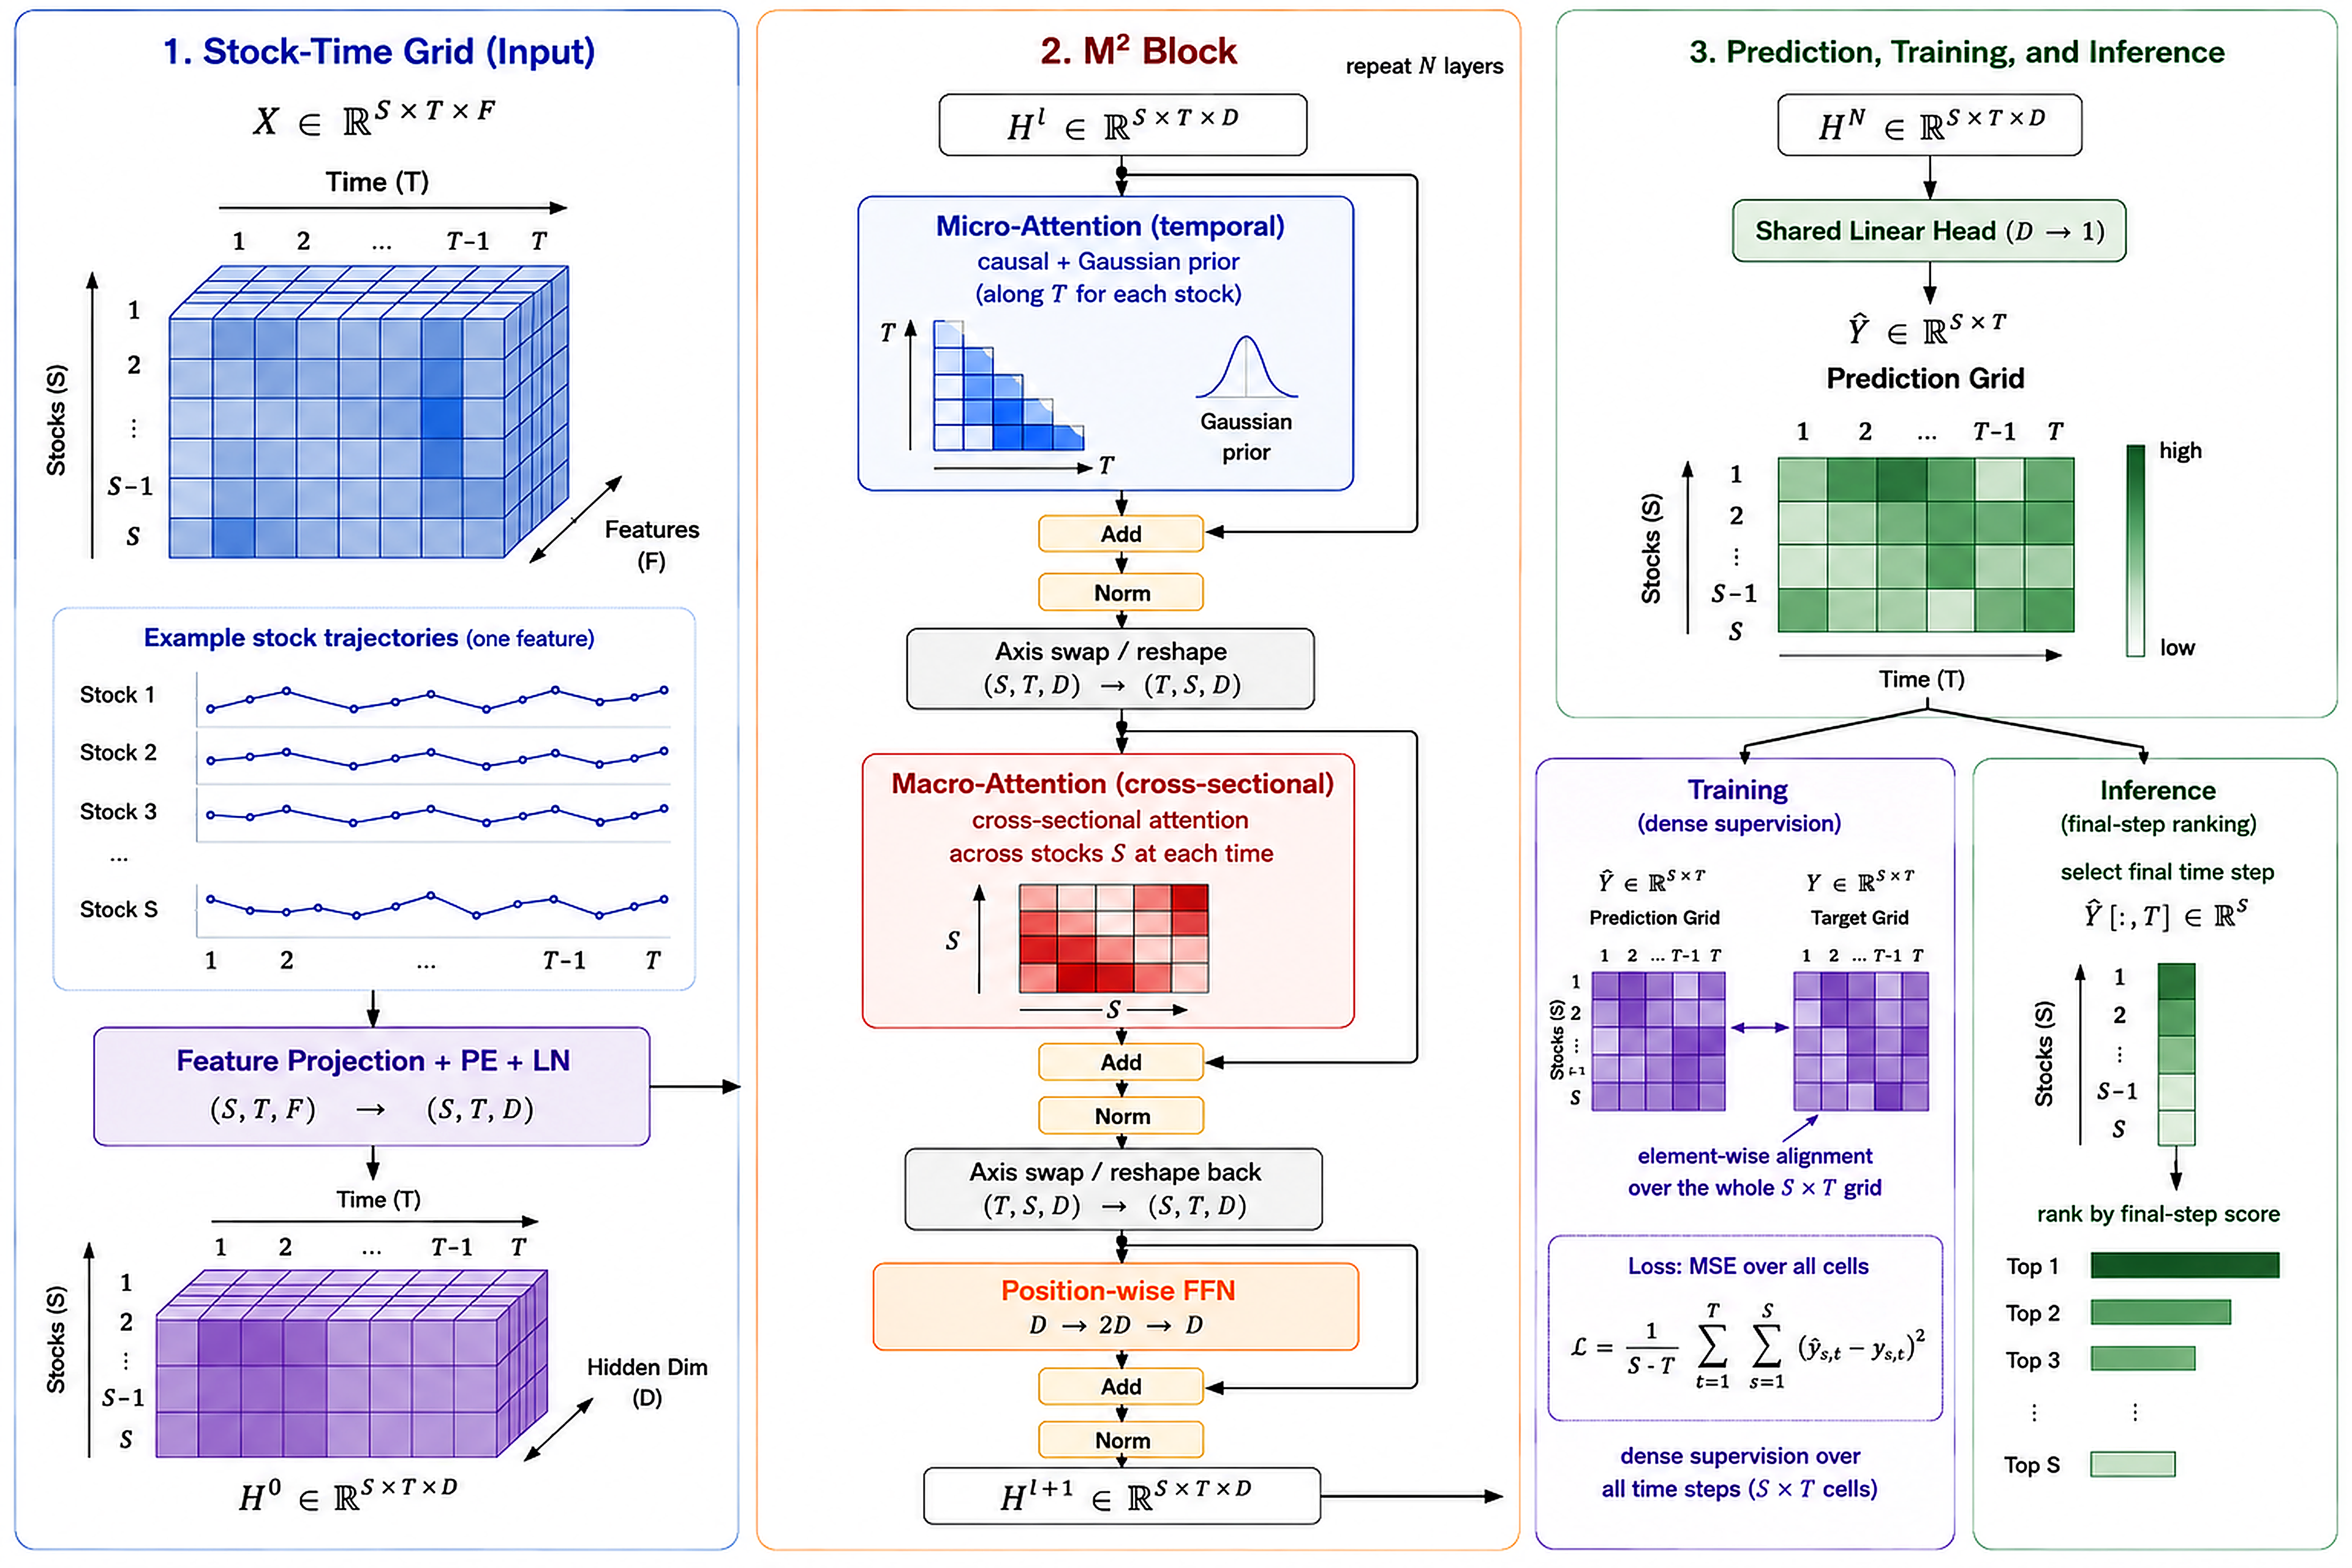
\includegraphics[width=\linewidth]{figures/fig_method.png}
\caption{Overall architecture of \msqa{}. Left: the input is a
stock $\times$ time $\times$ feature grid, mapped via feature projection $+$
positional encoding $+$ layer normalization to $\bm{H}^{(0)}$. Middle: $L$
\msq{} Blocks, each applying Micro (causal time-axis attention $+$ Gaussian
recency prior), Macro (cross-sectional-axis attention), and a position-wise
feed-forward FFN ($D\!\to\!2D\!\to\!D$), each sub-layer with residual $+$
normalization, transposing the tensor between the two axes. Right: a shared
linear head outputs a prediction grid $\hat{\bm{Y}}$ at each time step; at
training time the whole $S\times T$ grid is densely supervised, and at
inference the last-step scores are used to rank and select.}
\label{fig:method}
\end{figure}

\subsection{Design motivation: dual-axis dependence and iterative re-reading}\label{sec:m-intuition}
Judging whether a stock is worth buying usually relies on two kinds of
information along the two axes: the stock's \emph{own recent trajectory} (time
axis), and its \emph{relative position in the whole market today} (cross-section
axis). Looking only at the trajectory ignores whether the current market regime
favors this type of stock; looking only at the cross-sectional position loses
whether it has been accelerating or has just peaked.

More importantly, these two kinds of information are \emph{interdependent}: to
judge ``where it ranks today,'' one must first understand each stock's own
trajectory, otherwise the cross-sectional position has no semantics; to read
``what this trajectory means,'' one must reference the same-day market
context---the same drop means opposite things in a crash versus a bull market.
A single sequential pass (finishing one axis before the other) cannot unlock
this circular dependence: when the time axis is processed first the
cross-sectional context is unknown, and when the cross-section axis is
processed first it operates on a temporal representation not yet calibrated by
the cross-section.

We therefore use $L$ structurally identical Blocks to let the dual axes
\emph{iteratively} re-read each other: the cross-sectional information output by
Macro at layer $\ell$ flows through the residual connection into Micro at layer
$\ell{+}1$, letting the latter re-read the stock's temporal trajectory under
the now-known same-day market context; Macro at layer $\ell{+}1$ in turn takes
this context-calibrated temporal representation and updates the cross-sectional
position again. Here ``combination'' is structural (both axes run),
``iteration'' is behavioral (each pass re-reads the previous pass's output
rather than recomputing). Whether the stacking gain indeed comes from this
iterative behavior, rather than simply from more parameters, is tested
experimentally in \S\ref{sec:depth}.

\subsection{Input representation and feature projection}\label{sec:m-input}
Let the input to a trading cross-section be
$\bm{X}\in\mathbb{R}^{S\times T\times F}$: $S$ stocks, a lookback window of $T$
trading days, and $F$ features per day (notation summary in
Table~\ref{tab:notation}). A per-(stock, time) shared linear projection maps
the feature dimension to the model dimension $D$, sinusoidal positional
encodings $\bm{P}$ along the time axis are added, and layer normalization gives
the initial hidden representation
\begin{equation}\label{eq:input}
\bm{H}^{(0)} = \mathrm{LN}\big(\mathrm{Proj}(\bm{X}) + \bm{P}\big)\ \in\ \mathbb{R}^{S\times T\times D}.
\end{equation}
The default configuration feeds raw features $\bm{X}$ directly into the
projection.

\begin{table}[H]
\centering
\caption{Notation and symbols.}
\label{tab:notation}
\begin{tabularx}{\linewidth}{l>{\raggedright\arraybackslash}X}
\toprule
Symbol & Meaning \\
\midrule
$S,\ T,\ F,\ D$ & Number of stocks, lookback time steps, input feature dim, model hidden dim \\
$\bm{X}\in\mathbb{R}^{S\times T\times F}$ & Input panel (stock $\times$ time $\times$ feature) \\
$\bm{H}^{(\ell)}\in\mathbb{R}^{S\times T\times D}$ & Hidden representation at Block $\ell$ ($\ell=0,\dots,L$) \\
$\bm{H}^{(\ell)}_{s}\in\mathbb{R}^{T\times D}$ & Temporal slice of stock $s$ (Micro input) \\
$\bm{H}^{(\ell)}_{:,t}\in\mathbb{R}^{S\times D}$ & Cross-sectional slice at time step $t$ (Macro input) \\
$\bm{Q},\bm{K},\bm{V}$ & Query / key / value projections of attention; $d_k$ is per-head dim \\
$\sigma$ & Bandwidth of Micro's Gaussian recency prior (baseline $\sigma{=}4$) \\
$L$ & Number of stacked \msq{} Blocks (baseline $L{=}3$) \\
$\hat{\bm{Y}}\in\mathbb{R}^{S\times T}$ & Per-time-step cross-sectional prediction; last step $\hat{\bm{Y}}_{:,T}$ is the trading signal \\
\bottomrule
\end{tabularx}
\end{table}

\subsection{The \msq{} Block: dual-axis attention}\label{sec:m-block}
A \msq{} Block sequentially concatenates three sub-layers---Micro (causal
time-axis attention), Macro (cross-sectional-axis attention), and a
position-wise feed-forward FFN---each with a residual connection and
(post-)layer normalization. Let the input to layer $\ell$ be $\bm{H}^{(\ell)}$.

\comp{Micro (time axis, causal $+$ recency prior)}
Micro applies multi-head self-attention~\cite{transformer} on the time axis,
\emph{independently for each stock}, to capture its own trajectory. To prevent
information leakage the attention is constrained to be \emph{causal} (step $i$
attends only to history $j\le i$); borrowing the Gaussian prior idea from the
Gaussian Transformer~\cite{gausstransformer}, an additive \emph{time-distance
Gaussian prior} (single bandwidth $\sigma$, see below) is added to the
attention logits so that the model favors neighboring time steps. For stock
$s$, with representation sequence $\bm{H}^{(\ell)}_{s}\in\mathbb{R}^{T\times D}$,
\begin{equation}\label{eq:micro}
\mathrm{Micro}\big(\bm{H}^{(\ell)}_{s}\big)=\mathrm{softmax}\!\Big(\frac{\bm{Q}_s\bm{K}_s^{\top}}{\sqrt{d_k}}+\bm{B}\Big)\bm{V}_s,
\qquad
\bm{B}_{ij}=\begin{cases}\exp\!\big(-\dfrac{(i-j)^2}{2\sigma^2}\big), & j\le i,\\[8pt] -\infty, & j>i,\end{cases}
\end{equation}
where $\bm{Q}_s,\bm{K}_s,\bm{V}_s$ are linear projections of
$\bm{H}^{(\ell)}_{s}$. The lower-triangular entries of $\bm{B}$ are positive
biases decaying with temporal distance (the more recent past gets higher
weight), and the $-\infty$ on the upper triangle implements causal masking.

\comp{Macro (cross-section axis, soft consensus)}
Macro lets all stocks apply multi-head self-attention to each other
\emph{independently at each time step}, capturing each stock's same-day
relative position in the whole market. In implementation the tensor is
transposed between the stock axis and the time axis; for the cross-section
$\bm{H}_{:,t}\in\mathbb{R}^{S\times D}$ at time step $t$,
\begin{equation}\label{eq:macro}
\mathrm{Macro}\big(\bm{H}_{:,t}\big)=\mathrm{softmax}\!\Big(\frac{\bm{Q}_t\bm{K}_t^{\top}}{\sqrt{d_k}}\Big)\bm{V}_t.
\end{equation}
No mask is applied here---every stock can attend to all stocks on the same day,
yielding a kind of \emph{soft consensus} across the cross section, rather than
a hard relation graph based on industry or supply chain. \S\ref{sec:macro}
analyzes through interpretability experiments what Macro actually learns and
provides support for this design choice.

\comp{FFN, residual, and normalization}
Finally a per-(stock, time) position-wise feed-forward network
$\mathrm{FFN}(\bm{h})=\bm{W}_2\,\mathrm{ReLU}(\bm{W}_1\bm{h})$ is applied, with
$\bm{W}_1:\mathbb{R}^{D}\!\to\!\mathbb{R}^{2D}$ and
$\bm{W}_2:\mathbb{R}^{2D}\!\to\!\mathbb{R}^{D}$. All three sub-layers use
residual $+$ post-normalization:
\begin{equation}\label{eq:residual}
\bm{H}\ \leftarrow\ \mathrm{LN}\big(\bm{H}+\mathrm{Sublayer}(\bm{H})\big),\qquad
\mathrm{Sublayer}\in\{\mathrm{Micro},\ \mathrm{Macro},\ \mathrm{FFN}\},
\end{equation}
applied in turn Micro, Macro, FFN to obtain this layer's output
$\bm{H}^{(\ell+1)}$.

\subsection{Stacking and iterative refinement}\label{sec:m-stack}
$L$ structurally identical Blocks are stacked,
$\bm{H}^{(\ell+1)}=\mathrm{Block}\big(\bm{H}^{(\ell)}\big)$,
$\ell=0,\dots,L-1$. Because each sub-layer has a residual connection, Micro at
layer $\ell{+}1$ already accumulates the cross-sectional information injected
by Macro at layer $\ell$: it no longer processes the ``bare'' raw temporal
sequence but re-reads the stock's temporal trajectory under the now-known
same-day market context---this is exactly the iterative re-reading described
in \S\ref{sec:m-intuition}. Stacking is therefore not repeating the same
computation $L$ times but letting the two interdependent views alternate and
converge on the residual channel.

A natural worry: is the stacking gain just from having more parameters? We rule
this out with two controls in \S\ref{sec:depth}. First, widening the
representation dimension $D$ (adding parameters but not iterative layers):
returns saturate quickly ($D{=}128$ ties $256$) and never reach the height
gained by deepening. Second, sweeping the stacking depth $L\in[1,5]$:
deepening keeps lifting, just with diminishing returns, consistent with
``iterative per-layer refinement with diminishing gains'' rather than ``more
parameters are better.''

The stacking process never flattens the time dimension; the $(S,T,D)$
representation runs through end to end, preserving full information for the
per-time-step dense supervision.

\subsection{Prediction head, labels, and training objective}\label{sec:m-head}
The last-layer representation $\bm{H}^{(L)}$ is mapped to a scalar by a linear
head shared across all (stock, time) positions, giving the prediction grid
\begin{equation}\label{eq:head}
\hat{\bm{Y}} = \bm{H}^{(L)}\bm{w} + b\ \in\ \mathbb{R}^{S\times T}.
\end{equation}
Each element $y_{s,t}$ of the label $\bm{Y}\in\mathbb{R}^{S\times T}$ is the
\emph{next-day cross-sectional $z$-scored return} of stock $s$ on day $t$
(standardized within the same-day cross section so that the supervision signal
itself is ``relative strength'' rather than absolute move). At training time
\emph{dense supervision} is applied over the entire $S\times T$ grid, and the
baseline uses mean-squared error,
\begin{equation}\label{eq:loss}
\mathcal{L}=\frac{1}{S\,T}\sum_{s=1}^{S}\sum_{t=1}^{T}\big(\hat{y}_{s,t}-y_{s,t}\big)^2 .
\end{equation}
Dense supervision turns every time step in the window into a training signal,
substantially increasing gradient density. At inference only the last-step
score $\hat{\bm{Y}}_{:,T}\in\mathbb{R}^{S}$ is taken as the day's trading
signal; stocks are ranked descending by score and the top few form the holdings
(backtest protocol in \S\ref{sec:setup}). Beyond MSE, we systematically compare
ranking and classification losses and other training objectives in
\S\ref{sec:objective}.

\subsection{Implementation details and default configuration}\label{sec:m-impl}
\textbf{Model.} The baseline configuration is: lookback window $T{=}8$
trading days, model dim $D{=}128$, $L{=}3$ stacked layers, Micro heads $4$ /
Macro heads $2$, FFN expansion ratio $2$, dropout $0.1$, Gaussian bandwidth
$\sigma{=}4$, sinusoidal positional encoding, post-norm, intra-block order
Micro$\to$Macro. The default \emph{does not} use an industry prior (industry
attention); the industry prior, together with PE variants, sparse Macro, etc.,
is discussed as a variant in \S\ref{sec:exp} and the appendix. The market vector
is obtained by aggregating 3 market indices (SSE Composite, CSI 300, ChiNext)
over 5 lookback scales and is enabled only in variants that use market
information. Weights use Xavier initialization.

\textbf{Training.} One trading day's all stocks form a batch; the
optimizer is AdamW (learning rate $10^{-5}$, weight decay $10^{-4}$); gradients
are clipped by norm to $5.0$; the baseline uses no learning-rate schedule
(scheduling policies appear as an appendix ablation). Training runs up to $40$
epochs with \emph{validation-IC} early stopping (patience $=10$). Each
configuration is trained independently with 3 random seeds (42 / 123 / 2024).
Data splitting, normalization, and the no-leakage treatment are in
\S\ref{sec:setup}.

% ================================================================ 5 Experiments
\section{Experiments}\label{sec:exp}

% ---------------- 5.1
\subsection{Setup and the unified evaluation protocol}\label{sec:setup}

\textbf{Data and task.} Data sources, the stock universe, the feature
pipeline, normalization, and the no-leakage label construction have been stated
uniformly in \S\ref{sec:data} (overview in Table~\ref{tab:pipeline}): about
$35$ price-volume / fundamental / money-flow features, per-day cross-sectional
robust $z$-score, cross-sectional ranking labels, and a temporal split into
train 2017-01\,$\sim$\,2023-12 / valid 2024-01\,$\sim$\,2025-06 / test
2025-07\,$\sim$\,2026-05. This section only adds the backtest and evaluation
protocol.

\textbf{Backtest and evaluation.} Training is on CSI 300 constituents;
the backtest is on the $\sim$1000 most liquid stocks (top1000; illiquid ST
stocks and Beijing Stock Exchange stocks already removed). The trading
strategy follows the unified backtest template plus a diversification
constraint (hereafter \emph{our backtest strategy}): equal-weight holding of
$n{=}10$ names, each day buying from the top-100 by prediction score and
selling holdings that drop out of the top-200, a $20\%$ cap on any single
industry, open-price execution, a round-trip fee of $0.13\%$, and an initial
capital of 1,000,000 CNY. Prediction quality is measured by IC (the information
coefficient, the cross-sectional correlation between same-day prediction and
next-day realized return), RankIC (its rank-correlation version), and ICIR (the
mean / std of the IC series, measuring stability); the backtest reports
cumulative return, annualized return, Sharpe, and max drawdown, compared
against market indices (SSE Composite, CSI 300) and a simple MLP baseline
(\S\ref{sec:main}). Fig.~\ref{fig:loss} shows the baseline's train / validation
loss: training loss drops steadily while validation loss is roughly flat---a
common shape for low-SNR financial data, and a harbinger that validation-side
metrics will decouple from out-of-sample performance (\S\ref{sec:select}).

\begin{figure}[H]
\centering
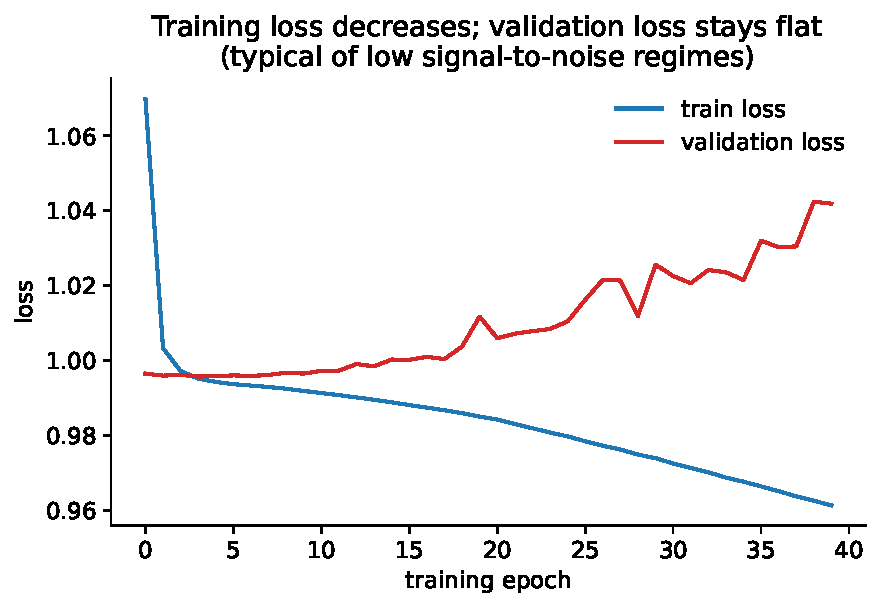
\includegraphics[width=0.62\linewidth]{figures/fig_loss.pdf}
\caption{Training and validation loss of the baseline over epochs. Training
loss drops steadily while validation loss is roughly flat---a common shape
under low-SNR financial data, also foreshadowing the decoupling of
validation-side metrics from out-of-sample performance (\S\ref{sec:select}).}
\label{fig:loss}
\end{figure}

\textbf{Unified evaluation protocol.} Every configuration reports two
numbers at once. \textbf{(i) Best ckpt}\bestckpt{}: among the per-epoch saved
checkpoints, take the one with the highest \emph{test} return; it uses
information from the test set that should not be visible, so it is an oracle
upper bound that only measures the capability ceiling and across-seed stability
and is not deployable. \textbf{(ii) Validation-selected checkpoint}: pick the
checkpoint on the validation set---this is the honest, deployable number. Key
conclusions always report multi-seed $\text{mean}\pm\text{std}$ (seeds
42/123/2024) and set a \textbf{variance redline} of $\approx\pm 60$pp---the
order of magnitude of return swings that the same configuration can produce
solely from seed and checkpoint choice (see \S\ref{sec:select}); differences
below the redline are treated as noise. \textbf{Decision rule.} We
uniformly use \emph{error bar $=$ multi-seed $\text{mean}\pm1\,\text{std}$}
($n{=}3$): two configurations are considered a genuine difference beyond seed
noise only when their error bars \emph{do not overlap}; otherwise they are
treated as same-order noise. Note that $n{=}3$ is small, so this is
\emph{engineering judgment} rather than a strict statistical test, supporting
only qualitative conclusions of ``clearly separated.'' Also, \bestckpt{} takes
the test-best on the \emph{saved} checkpoint grid; if different configurations
have grids of different densities, their comparability is reduced---so we
downgrade comparisons of unequal grids to \emph{corroborating} evidence (e.g.\
Appendix~\ref{sec:abl-dense}) and take as the primary judgment those
comparisons whose grids match or which use the validation-selected protocol.
Table~\ref{tab:protocol} is the reading template for base under the two
protocols.

\begin{table}[H]
\centering
\caption{Reading template under the unified evaluation protocol (using base as
the example). \bestckpt{} $=$ best ckpt (upper bound).}
\label{tab:protocol}
\begin{tabular}{lcccc}
\toprule
Configuration & seed42 & seed123 & seed2024 & mean$\pm$std \\
\midrule
base (best ckpt\bestckpt)  & +170.9\% & +166.0\% & +128.6\% & $+155\pm19$\% \\
base (validation-selected) & +55\%    & +117\%   & $-3$\%   & \msd{+56}{60}\% \\
\bottomrule
\end{tabular}
\end{table}

% ---------------- 5.2
\subsection{Checkpoint-selection failure and across-seed variance}\label{sec:select}
On a low-SNR cross-sectional task, simply changing the random seed or the
checkpoint for the same configuration can move the return by hundreds of
percentage points. The magnitude of this noise is the premise for interpreting
every architectural comparison: differences smaller than it cannot distinguish
``genuine effect'' from ``different seed.''

\textbf{Setup.} We run two controls on the baseline ($L{=}3$, $D{=}128$,
$\sigma{=}4$) under the same backtest protocol as \S\ref{sec:setup} (top1000
universe, open-price execution, round-trip fee $0.13\%$, test period 2025-07 to
2026-05). The first fixes seed42, saves a checkpoint every epoch, and backtests
each, examining whether the within-run return trajectory over epochs moves in
the same direction as validation IC; the second fixes all other configurations
and changes only the seed (42 / 123 / 2024), taking numbers under both the
\emph{validation-selected} and \emph{best-ckpt} rules to measure seed-induced
swings.

\textbf{Results.} Within a single run, validation IC rises monotonically
with epoch ($0.020\to0.027$), while test return peaks at ep13 and then keeps
declining; their Pearson correlation is $-0.75$ (Fig.~\ref{fig:ic-return}).
Picking the checkpoint by ``highest validation IC'' selects ep34---the worst
out-of-sample end---whereas the genuinely best ep13 has an unremarkable
validation IC. Varying only the seed, the validation-selected returns are
$-3\%$, $+55\%$, $+117\%$ (mean $+56\%$, std $\pm60$pp); switching the same
three seeds to best-ckpt gives $+171\%$ / $+166\%$ / $+128\%$ (mean $+155\%$,
std narrowing to $\pm19$pp). The $-3\%$ of seed2024 is not because the model is
worse, but because that run's validation-selected checkpoint happened to land
on a poorly generalizing point.

\textbf{Analysis.} Three points follow. First, validation IC cannot be
used to select checkpoints---it inversely relates to out-of-sample return, so
conventional early stopping backfires here. More generally: in such a low-SNR
regime, a metric going up is itself often a signal of overfitting, not of
stronger capability---the validation segment is short and noisy, and late-epoch
IC gains are mostly the model fitting validation noise (consistent with the
flat validation loss in Fig.~\ref{fig:loss}). At high noise levels, a
point-estimate correlation like IC is no longer a reliable proxy for
``out-of-sample capability''; ``more accurate'' does not imply ``more
profitable.'' Second, the combined seed-plus-selection swing of about $\pm60$pp
exceeds the effect of most architectural changes that follow. These two points
set the reading rule for the entire paper: key conclusions always report
best-ckpt $+$ multi-seed mean$\pm$std, and configurations differing by less
than $\pm60$pp are treated as noise with no claim of superiority---much of the
``architectural gains'' reported in the literature from single runs likely fall
within this redline. Third, since the metric itself can deceive within noise,
``what to optimize during training and what to trust at deployment'' must be
decided by context, not by blindly maximizing IC: \S\ref{sec:objective} will
show that losses directly targeting ranking (IC-style objectives) actually have
larger variance, while regression and classification are the stable ones. The
return distribution of each configuration is shown in Fig.~\ref{fig:variance}.

\begin{figure}[H]
\centering
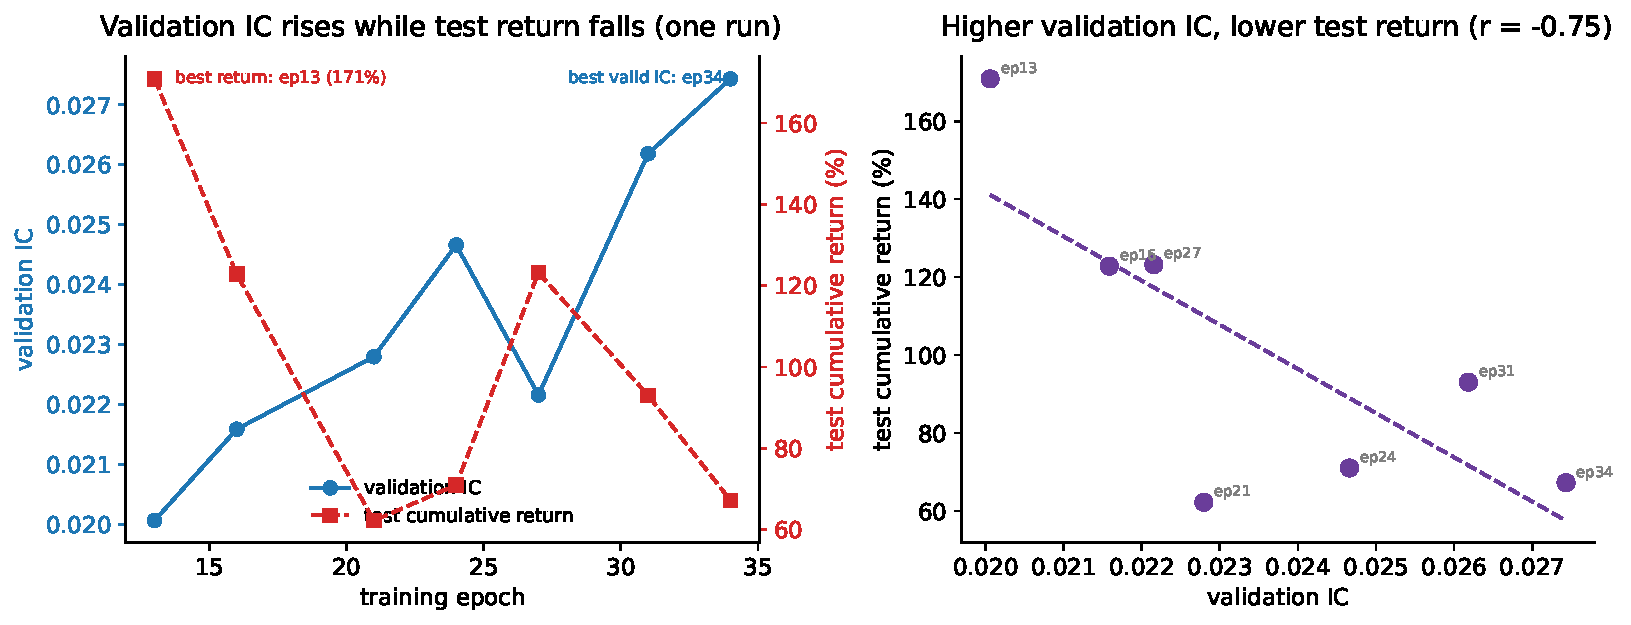
\includegraphics[width=\linewidth]{figures/fig_ic_return.pdf}
\caption{Inverse relation between validation IC and out-of-sample return
(baseline, seed42). Left: within a single run over epochs, validation IC keeps
rising while test cumulative return peaks early and then declines. Right: each
checkpoint as a point---the higher the validation IC, the lower the
out-of-sample return (Pearson $r=-0.75$); the ``highest-validation-IC'' pick
(ep34) happens to fall on the worst-return end.}
\label{fig:ic-return}
\end{figure}

\begin{figure}[H]
\centering
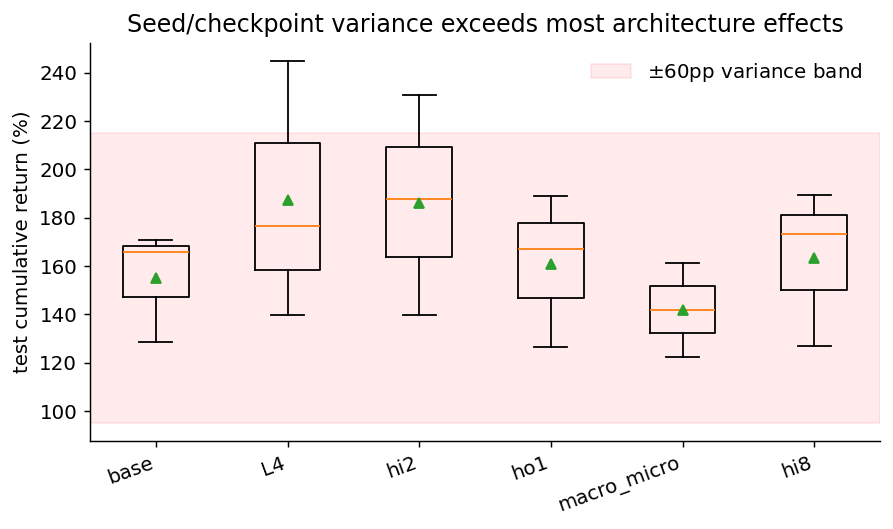
\includegraphics[width=0.92\linewidth]{figures/fig_variance.png}
\caption{Best-ckpt return distribution of each configuration over seeds
(box plots; triangles are means), overlaid with the $\pm 60$pp variance-redline
band centered on base. Base and most architectural variants (deeper stacking,
different Micro / Macro head counts, swapped sub-layer order) overlap across
seeds and all fall within the redline band---the differences between
configurations are largely indistinguishable from seed noise.}
\label{fig:variance}
\end{figure}

% ---------------- 5.3
\subsection{Main comparison and failure diagnosis}\label{sec:main}

\subsubsection{Main comparison}\label{sec:main-cmp}
\textbf{Setup.} Thirteen representative methods are compared with
\msqa{} on the same panel: the same $35$ features, the same data split, the
same backtest strategy (\S\ref{sec:setup}), test period 2025-07 to 2026-05.
The baselines are trained by their original settings and report the
single-seed (seed42) validation-selected result, while \msqa{} reports
best-ckpt. CSI 300 buy-and-hold is the market benchmark, and a per-point MLP
(that models no temporal or cross-sectional relation) is the ``no-structure''
lower bound.

\textbf{Results.} \msqa{} (best ckpt) leads with $+170.9\%$, Sharpe
$2.99$ (Table~\ref{tab:main}). Next come the training paradigms designed for
low SNR---RSR $+94.5\%$, adversarial AdvALSTM $+78.9\%$, TRA $+63.2\%$;
classical temporal models (Transformer / LSTM / ALSTM / GRU) fall in
$+20\%\sim+49\%$; finance-specialized models converted to cross-sectional
ranking (HIST / MASTER / DTML / SFM) are at the bottom, $+3\%\sim+23\%$.
CSI 300 buy-and-hold is $+24.8\%$: the training-paradigm school and \msqa{}
clearly beat the market, while GRU, MASTER, DTML, and SFM underperform even the
index.

\textbf{Analysis.} What ranks at the top are ranking / adversarial
paradigms designed for low SNR, not higher-capacity classical
architectures---returns come from task fit, not from piling up parameters. This
table cannot be read as a literal leaderboard: the baselines are single-seed
and \msqa{} is an oracle upper bound, the protocols are asymmetric, and
single-seed returns themselves jitter by $\pm60$pp (\S\ref{sec:select}). The
per-point MLP is the best reminder---it models no temporal or cross-sectional
relation yet still achieves $+98.3\%$ under best-ckpt, overtaking most
specialized baselines; under an oracle ceiling, strong features plus
checkpoint selection already explain a substantial portion of the return. So
this table should be read only as a capability comparison under the oracle
upper bound; multi-seed, deployable-protocol per-item results appear in
\S\ref{sec:pillars} onward.

\begin{table}[H]
\centering
\caption{Main comparison: unified backtest protocol (our backtest strategy,
seed42). \msqa{} reports best ckpt (upper bound); baselines are single-seed.}
\label{tab:main}
\begin{tabular}{llccc}
\toprule
Family & Model & Test cumulative & Sharpe & Max drawdown \\
\midrule
\textbf{Ours} & \textbf{\msqa{} (best ckpt)} & \textbf{+170.9\%} & \textbf{2.99} & $-14.7\%$ \\
\midrule
\multirow{3}{*}{Training-paradigm school}
 & RSR        & +94.5\% & 2.07 & $-22.3\%$ \\
 & AdvALSTM   & +78.9\% & 2.10 & $-27.0\%$ \\
 & TRA        & +63.2\% & 1.63 & $-18.3\%$ \\
\midrule
\multirow{4}{*}{Classical temporal}
 & Transformer & +48.8\% & 1.49 & $-14.1\%$ \\
 & LSTM        & +37.9\% & 1.52 & $-14.7\%$ \\
 & ALSTM       & +33.8\% & 0.91 & $-36.4\%$ \\
 & GRU         & +20.2\% & 1.17 & $-10.7\%$ \\
\midrule
\multirow{4}{*}{Finance-specialized}
 & HIST   & +23.2\% & 0.79 & $-28.6\%$ \\
 & MASTER & +9.6\%  & 0.47 & $-37.4\%$ \\
 & DTML   & +4.9\%  & 0.36 & $-28.5\%$ \\
 & SFM    & +3.3\%  & 0.31 & $-34.7\%$ \\
\midrule
\multirow{2}{*}{Simple reference}
 & MLP (per-point, no temporal) & +98.3\% & 2.12 & $-17.1\%$ \\
 & CSI 300 index (buy-and-hold) & +24.8\% & 1.79 & $-7.8\%$ \\
\bottomrule
\end{tabular}
\end{table}

\subsubsection{Failure diagnosis}\label{sec:main-diag}
The finance-specialized models collectively sit at the bottom; one possibility
is that they degrade when converted to a cross-sectional ranking objective.

\textbf{Setup.} We faithfully reproduce the three models by their
respective original objectives and signals---MASTER with 5-day return MSE, DTML
with up/down BCE, SFM with per-stock price MSE---and evaluate them under the
same backtest protocol (Table~\ref{tab:faithful}).

\textbf{Results.} Under the faithful objectives the three remain low
(Table~\ref{tab:faithful}): MASTER $-19.8\%$, DTML $+4.5\%$, SFM $+9.0\%$, as
poor as their ranker-converted versions in Table~\ref{tab:main}. The key signal
is the negative result: it is not the backtest protocol or fees eating the
return---their throughout-validation IC stays glued between $-0.01$ and $0$
(MASTER $-0.011\sim-0.006$, DTML $-0.008\sim-0.002$, SFM $-0.005\sim-0.001$),
roughly zero, slightly negative; that is, the prediction score is almost
uncorrelated with the next-day cross-sectional return. IC$\approx 0$ means they
have essentially learned no usable cross-sectional signal in A-shares.

\textbf{Analysis.} Since faithfully reproducing them by their respective
paper objectives (not converting to a ranker) still gives IC near zero, the
``objective was broken by conversion'' explanation is ruled out; the failure
lies in a structural mismatch between the architecture and the task---their
objectives and inductive biases are inherently ill-suited to A-share low-SNR
cross-sectional ranking. One by one: \textbf{MASTER} ($-19.8\%$, the only loss)
relies on market-guided gating that modulates per-stock representation by
overall market state, but A-share market factors are noisy and regimes switch
fast, so the gating easily locks onto spurious market signals and amplifies
noise as structure---this mirrors \S\ref{sec:macro}: Macro works because it
converges to a few robust co-rise/co-fall clusters, while MASTER takes the
``whole-market mean'' as an anchor and anchors the wrong way. \textbf{DTML}
($+4.5\%$) uses up/down binary BCE as the training target, but A-share daily
up/down is close to 50/50 and a binary label carries almost no information,
analogous to the direct collapse of BCE to $-6\%$ in \S\ref{sec:objective}; the
label itself has lost the cross-sectional strength signal.
\textbf{SFM} ($+9.0\%$) does frequency decomposition plus per-stock price MSE,
which presumes decomposable stable periodic components in stock prices; A-share
prices are non-stationary with large stock-specific noise, so what gets
decomposed is mostly noise harmonics, and per-stock MSE optimizes single-stock
price fitting, orthogonal to cross-sectional relative ranking. The failures of
all three converge to the same conclusion: on a low-SNR cross-sectional ranking
task, only ranking / adversarial paradigms with explicit strength signals (the
training-paradigm school in Table~\ref{tab:main}) work; these architectures
designed for other objectives do not transfer.

\textbf{Boundary.} These are failures of out-of-the-box faithful
transfer (paper-default hyperparameters, single seed42), not proof that the
models are inherently bad---in their own original markets, periods, and
evaluation protocols the papers' results hold. The MASTER and DTML failure
modes have our own experimental corroboration (the Macro anchor in
\S\ref{sec:macro}, the BCE collapse in \S\ref{sec:objective}); the SFM line is
more of an architectural-principle inference, and we did not run a dedicated
frequency-decomposition ablation.

\begin{table}[H]
\centering
\caption{Faithful baselines (each model's own paper objective, seed42).}
\label{tab:faithful}
\begin{tabular}{lcc}
\toprule
Model (faithful objective) & Test cumulative & Sharpe \\
\midrule
MASTER (5-day return MSE) & $-19.8\%$ & $-0.34$ \\
DTML (up/down BCE)        & $+4.5\%$  & $+0.34$ \\
SFM (per-stock price MSE) & $+9.0\%$  & $+0.47$ \\
\bottomrule
\end{tabular}
\end{table}

% ---------------- 5.4
\subsection{Dual-axis ablation}\label{sec:pillars}
The model's capability rests on two axes: Micro reads a stock's own trajectory
along the time axis, Macro compares it with peers along the cross-section axis
(\S\ref{sec:method}). If the design holds, removing either axis should
noticeably reduce the return; if one axis is in fact redundant, removing it
should leave the return unchanged or even higher.

\textbf{Setup.} Two ways of removal. Removing the Macro cross-section
axis eliminates cross-stock interaction, and the model degenerates into a
single-stock sequence model along the time axis only; replacing Micro's causal
self-attention with a unidirectional LSTM keeps the time axis but changes the
reading from ``global attention within the window'' back to ``day-by-day
recurrence.'' All other configurations, data splits, and backtest protocol are
the same as base; each variant runs seeds 123/2024 and reports best-ckpt
(protocol in \S\ref{sec:select}).

\textbf{Results.} Both axes are indispensable (Table~\ref{tab:pillars},
Fig.~\ref{fig:pillars}). Base is $+155\pm19\%$; turning off Macro drops it to
$+109\pm7\%$ ($-46$pp); replacing Micro with LSTM drops it to $+111\pm10\%$
($-44$pp). These $\sim 45$pp drops are of the same order as the seed-variance
redline ($\pm60$pp), so a single run cannot tell true from false; but under the
best-ckpt multi-seed protocol both variants are below base and their error bars
do not overlap with base---a genuine effect. Under the validation-selected
protocol, some seeds of Macro-off pick poorly generalizing checkpoints and
returns go as low as near zero (the same mechanism by which base's
validation-selected seed2024 lands at $-3\%$, \S\ref{sec:select}); this is a
selection artifact, not the model truly going to zero; switching to the
best-ckpt protocol shows it sits stably at $+109\%$, systematically below base
but far from zero.

\textbf{Analysis.} Each axis, when removed, has a traceable mechanism
for the loss. The mechanism for removing Macro is developed in detail in
\S\ref{sec:macro}: Macro's job is to pull overly extreme predictions toward the
cross-sectional consensus ($59\%$ of stocks are pulled closer to the industry
mean); without it, a stock's extreme score is no longer corrected by peers, and
the ranking is more easily led astray by single-stock noise. The drop from
replacing Micro with LSTM is comparable, but the difference is in how the time
axis is read---causal self-attention lets any day in the window look directly
back at any earlier day, while LSTM can only compress history into a hidden
state carried forward, with distant information decaying along the way. One
confound to rule out: replacing with LSTM also discards Micro's Gaussian
recency prior; but removing the Gaussian prior alone leaves the return within
the noise band (Appendix~\ref{sec:abl-micro}), so this $44$pp is mainly charged
to ``how the time axis is read,'' not to the Gaussian prior. After removing
either axis, the error bars separate from base and the mechanisms are
independently traceable, indicating that the two axes are not redundant backups
but true pillars on each of which return depends.

\begin{table}[H]
\centering
\caption{Dual-axis pillar ablation (test cumulative return, best ckpt,
multi-seed). All three configurations use seeds 42/123/2024 ($n{=}3$); the
error bars of Macro-off and Micro-replaced-by-LSTM do not overlap with base.}
\label{tab:pillars}
\begin{tabular}{lcccc}
\toprule
Configuration & seed42 & seed123 & seed2024 & mean$\pm$std \\
\midrule
base (full)              & $+170.9$ & $+166.0$ & $+128.6$ & $\mathbf{+155\pm19}$ \\
Macro off (no cross-section) & $+105.9$ & $+119.2$ & $+102.3$ & $+109\pm7$ \\
Micro $\to$ LSTM         & $+121.5$ & $+97.6$  & $+115.2$ & $+111\pm10$ \\
\bottomrule
\end{tabular}
\end{table}

\begin{figure}[H]
\centering
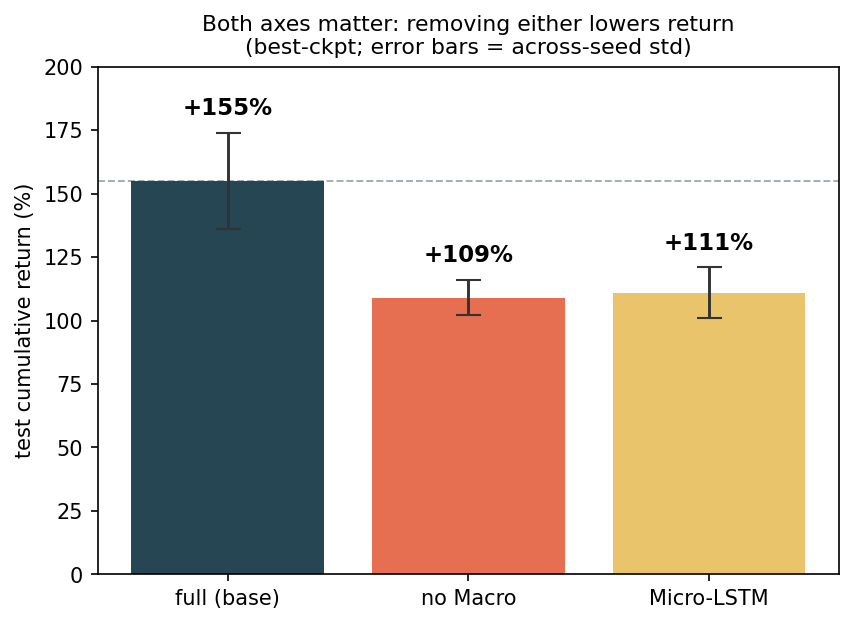
\includegraphics[width=0.62\linewidth]{figures/fig_pillars.png}
\caption{Dual-axis pillars (best ckpt; error bars are seed standard
deviations). After turning off Macro or replacing Micro with LSTM, the return
error bars do not overlap with base---the decline is a genuine effect beyond
seed noise.}
\label{fig:pillars}
\end{figure}

% ---------------- 5.5
\subsection{Stacking depth}\label{sec:depth}
\S\ref{sec:m-stack} uses stacked \msq{} Blocks to let the dual axes
iteratively re-read each other. The stacking gain could come from this
iteration or just from more layers and parameters; a depth sweep separates the
two explanations.

Using the notation of \S\ref{sec:m-stack}, ``iteration'' can be written
explicitly: starting from the input representation $\bm{H}^{(0)}$, depth $L$ is
the number of times the same Block is repeatedly applied,
\begin{equation}\label{eq:iter}
\bm{H}^{(L)}=\underbrace{\mathrm{Block}\circ\cdots\circ\mathrm{Block}}_{L\ \text{layers}}\big(\bm{H}^{(0)}\big),
\qquad
\bm{H}^{(\ell+1)}=\mathrm{Block}\big(\bm{H}^{(\ell)}\big)=\mathrm{FFN}\!\big(\mathrm{Macro}\,(\mathrm{Micro}(\bm{H}^{(\ell)}))\big),
\end{equation}
with residual on every sub-layer. The point is that residual lets the two axes
alternately ``re-read'' the other's latest conclusion: Micro at layer $\ell{+}1$
reads an $\bm{H}^{(\ell)}$ that has already accumulated the cross-sectional
context injected by the previous Macro, and Macro at this layer in turn reads
the temporal representation just refined by Micro. So adding a layer is not
recomputing the same mapping one more time but letting Micro / Macro iterate
one more round on each other's latest output, refining $\bm{H}$ layer by
layer---$L$ directly controls ``how many rounds of re-reading.'' The depth
experiment sweeps exactly this $L$.

\textbf{Setup.} Fix all other configurations ($D{=}128$, $\sigma{=}4$,
Micro / Macro head counts and base architecture unchanged), vary only the
stacking depth $L\in\{1,2,3,4,5\}$, train each $L$ with 3 seeds, and backtest
per epoch to take best ckpt. To separate ``iteration'' from ``more
parameters,'' we add a sweep over the representation width $D$
($D\in\{64,128,256\}$, Appendix~\ref{sec:abl-arch}, also best-ckpt multi-seed)
as a control---widening is ``parameters only, no extra iterative layers''; if
the gain were mainly from capacity, widening should also keep rising.

\textbf{Results.} Table~\ref{tab:depth} and Fig.~\ref{fig:depth} give
the depth curve. Depth is beneficial overall: a single layer $L{=}1$ has the
lowest return ($+126\pm36\%$); from $L{=}2$ it jumps to the $+165\%$ range;
$L{=}4$ and $L{=}5$ rise further to $+187\%$ and $+201\%$. But the error bars
($\pm19$ to $\pm44$pp) overlap heavily; $L{=}3$ (base) is even slightly below
$L{=}2$ in mean; per-seed, $L{=}4$ beats $L{=}3$ on all three seeds, but
whether $L{=}5$ or $L{=}4$ is higher depends on the seed (on seed2024, $L{=}5$
is actually highest).

\textbf{Analysis.} The beneficial direction of depth is consistent with
the iteration hypothesis: each additional layer (one more iteration in
Eq.~\eqref{eq:iter}) lets Micro re-read the temporal sequence under the
cross-sectional context injected by the previous Macro, unlocking the mutual
dependence one layer further. The most telling point is the $L{=}1\to2$ jump
($+126\to+165$, $+39$pp, the largest step on the curve): with a single layer
each axis computes once without knowing the other's conclusion; at two layers,
Micro re-reads on Macro's cross-sectional context for the first time---iteration
goes from none to some, and return jumps a tier; this is the most direct
evidence that ``re-reading'' itself is at work, not just one more layer of
parameters. The gain flattens after $L{=}4$, consistent with ``iteration has a
convergence point''---a few alternating re-reads already suffice to unlock the
dependence; going deeper, the larger capacity tends to overfit under low SNR
and limited data, amplifying seed variance (the error bars widen with $L$).

Is the gain just from more layers and parameters? The widening control
(Appendix~\ref{sec:abl-arch}) gives negative corroboration: starting from base
($L{=}3$, $D{=}128$, $+155\%$) and adding the same batch of parameters in two
directions---in \emph{width} ($D{:}128\to256$) the return stays flat from
$+155\%$ to $+154\%$ (saturation, within the error bar); in \emph{depth}
($L{:}3\to4\to5$) it keeps rising to $+187\%$, $+201\%$. The same extra
parameters help when added to depth but not to width, indicating that the
depth gain is not ``more capacity'' per se but the extra round of dual-axis
re-reading that each new layer brings---exactly the design point of ``stacking
as iterative re-reading.'' Admittedly, the cleanest ``equal-parameter,
single-wide-layer vs.\ multiple-thin-layers'' control is left as future work.
This depth curve also falls inside the variance main thread---even a choice as
fundamental as stacking depth has an effect size comparable to seed / selection
noise (\S\ref{sec:select}).

\begin{figure}[H]
\centering
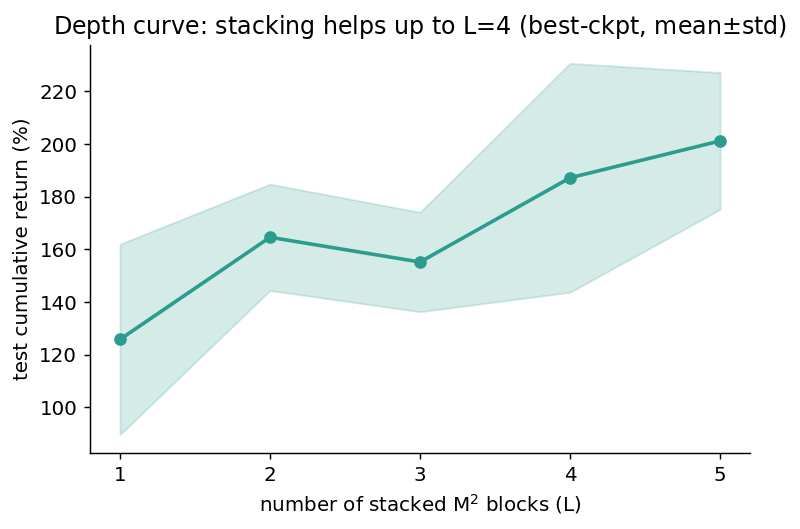
\includegraphics[width=0.62\linewidth]{figures/fig_depth.png}
\caption{Depth curve: test cumulative return vs.\ the number of stacked
\msq{} Block layers $L$ (best ckpt; shaded band is 3-seed mean$\pm$std).
Depth is beneficial overall ($L{=}1$ lowest, deeper higher), but the error
bars overlap heavily with no clean single sweet spot.}
\label{fig:depth}
\end{figure}

\begin{table}[H]
\centering
\caption{Depth curve (test cumulative return, best ckpt, 3-seed mean$\pm$std).}
\label{tab:depth}
\begin{tabular}{lcccc}
\toprule
Layers $L$ & seed42 & seed123 & seed2024 & mean$\pm$std \\
\midrule
L1 & $+75.0$  & $+156.7$ & $+145.7$ & $+126\pm36$ \\
L2 & $+145.6$ & $+155.6$ & $+192.6$ & $+165\pm20$ \\
L3 (base) & $+170.9$ & $+166.0$ & $+128.6$ & $+155\pm19$ \\
L4 & $+245.0$ & $+176.7$ & $+139.9$ & $+187\pm44$ \\
L5 & $+191.5$ & $+175.4$ & $+236.8$ & $\mathbf{+201\pm26}$ \\
\bottomrule
\end{tabular}
\end{table}

% ---------------- Dense temporal supervision ablation
\subsection{Dense temporal supervision ablation}\label{sec:abl-dense}
Our second innovation---keeping the $(S,T,D)$ representation and applying dense
supervision at every time step in the window (\S\ref{sec:m-head},
\S\ref{sec:rw-sup})---contains two separable design decisions: the
\emph{representation design} (not flattening the time dimension) and the
\emph{objective design} (supervising all time steps rather than only the last).
This section runs a controlled ablation that isolates the \emph{objective
design} half: the architecture, inference path, hyperparameters, and seeds are
all unchanged (still outputting the full $\hat{\bm{Y}}\in
\mathbb{R}^{S\times T}$ and still taking only the last step at inference); the
sole change is restricting the summation range of the loss in
Eq.~\eqref{eq:loss} from the full window
\begin{equation}\label{eq:loss-dense}
\mathcal{L}_{\text{dense}}=\frac{1}{ST}\sum_{s=1}^{S}\sum_{t=1}^{T}\big(\hat y_{s,t}-y_{s,t}\big)^2
\quad\longrightarrow\quad
\mathcal{L}_{\text{last}}=\frac{1}{S}\sum_{s=1}^{S}\big(\hat y_{s,T}-y_{s,T}\big)^2 ,
\end{equation}
i.e., supervising only the last step. The only variable between the two arms is
therefore \emph{supervision density}, so we can judge whether ``per-time-step
dense supervision'' itself contributes---without confounding it with ``whether
the time dimension is retained.''

\textbf{Setup.} Both arms (dense / last-step) are trained independently
with the base configuration ($L{=}3$, $D{=}128$, $\sigma{=}4$, AdamW
$\text{lr}{=}10^{-5}$, $40$ epochs) under the same three seeds (42/123/2024);
the backtest protocol is as in \S\ref{sec:setup}. We report multi-seed
$\text{mean}\pm\text{std}$ under both the best-ckpt and validation-selected
protocols, against the $\pm60$pp variance redline (\S\ref{sec:select}). The
representation-design half (retain vs.\ flatten the time dimension, which
requires an additional time-pooling control) is beyond this controlled ablation
and left as future work (\S\ref{sec:discuss}).

\begin{table}[H]
\centering
\caption{Dense temporal supervision ablation (test cumulative return,
multi-seed). The two arms have identical architecture; the only variable is
supervision density (Eq.~\eqref{eq:loss-dense}). \textbf{Protocol caveat:} both
arms are \emph{independent re-runs} of this ablation (fixed $40$ epochs, unified
archive grid ep$4/8/\cdots/40$), where the dense arm is exactly the base
configuration; due to randomness and the archive grid (some seeds early-stop,
so grids are unequal in length), its absolute values are \emph{not exactly
equal} to the base in the main text ($+155\pm19$,
Tables~\ref{tab:protocol},~\ref{tab:pillars}, whose archiving protocol differs),
so this table is used only for the \emph{within-table} dense-vs-last relative
comparison and should not be reconciled directly with the main-text numbers.}
\label{tab:abl-dense}
\begin{tabular}{llcccc}
\toprule
Supervision & Protocol & seed42 & seed123 & seed2024 & mean$\pm$std \\
\midrule
\multirow{2}{*}{Dense (all steps, ours)} & best ckpt & $+166$ & $+129$ & $+59$ & $\mathbf{+118\pm44}$ \\
                        & valid-select & $+55$ & $+100$ & $-3$ & $\mathbf{+50\pm42}$ \\
\addlinespace
\multirow{2}{*}{Last-step only}      & best ckpt & $+19$ & $+69$ & $+49$ & $+45\pm21$ \\
       & valid-select & $+4$ & $+5$ & $+4$ & $+4.5\pm0.5$ \\
\bottomrule
\end{tabular}
\end{table}

\textbf{Results.} Dense supervision wins substantially \emph{under both
protocols} (Table~\ref{tab:abl-dense}): under validation-select, $+50\pm42$ vs.\
$+4.5\pm0.5$; under best ckpt, $+118\pm44$ vs.\ $+45\pm21$. The error bars in
both protocols \emph{do not overlap} (validation-select $[8.5,92.5]$ vs.\
$[4,5]$; best ckpt $[74,162]$ vs.\ $[25,66]$)---the advantage of dense
supervision exceeds the $\pm60$pp variance redline and is a genuine effect
rather than noise. Particularly striking is the last-step-only row: its three
seeds' validation-selected returns sit stably around $+4\%$ (std only $0.5$pp),
\emph{consistently} low.

\textbf{Analysis.} This confirms the \emph{objective design} half of the
second innovation: per-time-step dense supervision does contribute and is not
dispensable. The mechanism is direct---the window length is $T{=}8$, and dense
supervision makes each window produce $8\times$ the gradient signal of
``last-step-only,'' so the model learns more sufficiently; last-step-only
discards $7/8$ of the supervision signal and is severely undertrained, so the
cross-sectional ranking signal never stands up (validation-select sitting
stably at $+4\%$ is its manifestation). Two honest caveats. First,
\emph{validation-select} is the cleaner control (one ckpt per run, no
grid-size confound), and it alone gives a non-overlapping conclusion; the
best-ckpt protocol agrees in direction but has different early-stop points per
run and unequal archive grids (dense seed42 archived ep4--36, dense seed2024
early-stopped and archived only up to ep8), so it serves as
\emph{corroboration} rather than the primary judgment. Second, this ablation
fixes the $(S,T,D)$ representation across both arms and only varies supervision
density, isolating the \emph{objective design}; the \emph{representation
design} half (retain vs.\ flatten the time dimension) still needs a
time-pooling control and is left as future work (\S\ref{sec:discuss}).

% ---------------- 5.7
\subsection{Training-objective comparison}\label{sec:objective}
The task is cross-sectional ranking, so intuitively one might expect to
optimize a ranking loss directly rather than regressing returns. Switching the
training objective on the same backbone tests this intuition. Note that what is
compared here is the \emph{loss type} (regression / ranking / classification),
orthogonal to the \emph{supervision density} (dense vs.\ last step) of the
previous section.

\textbf{Setup.} Fixing the backbone and data, we only change the loss
and compare four families of objectives: regression (regression on
$z$-scored returns, base); ranking (SoftRank, a differentiable ranking loss
whose coefficient $\alpha$ controls how much of a regression term is
retained---$\alpha{=}0$ is pure ranking, and larger $\alpha$ leans more toward
regression); multi-class classification (slicing returns into ``strong up /
flat / strong down'' by strength); binary classification (up/down only, BCE).
Protocol as in \S\ref{sec:select}, best ckpt, multi-seed.

\textbf{Results.} Table~\ref{tab:objective}: stably in the base band are
regression ($+155\pm19$) and 3-class classification ($+151\pm8$), whose error
bars overlap. The two losses with a ranking term have much larger variance:
pure ranking ($\alpha{=}0$) $+105\pm29$ (three seeds $73 / 98 / 143$);
ranking$+$regression mix ($\alpha{=}50$) $+131\pm43$ (three seeds
$70 / 163 / 161$---two seeds reach the $+160$ range, one training run diverges
and reaches only $+70$). The only direct collapse is binary classification,
$-6\%$.

\textbf{Analysis.} Although the task is cross-sectional ranking,
directly optimizing a ranking loss neither raises the mean nor amplifies
variance less. Pure ranking ($\alpha{=}0$) uses only the \emph{order} between
samples and discards the \emph{magnitude of return difference}---under low SNR
this magnitude is not redundant; it tells the model which contrasts are
high-confidence and worth learning more, and that is why pure ranking has the
lowest mean. The mixed loss ($\alpha{=}50$) adds the regression term back and
lets good seeds reach the $+160$ range, but it is also more prone to training
divergence (seed42 only reaches $+70$); its overall variance is clearly larger
than pure regression (std $43$ vs.\ $19$, about $2\times$). What is truly stable
is the two losses that feed strength information in a stable way---regressing
the $z$-score and 3-class classification---which sit stably in the base band.
This is consistent with the main thread of the paper: even the difference
brought by ``which training objective to use'' is mostly drowned in seed
variance.

The collapse of binary classification is the extreme version of the same
logic. ``Up / down'' compresses each stock into one bit, losing both the
magnitude and the fine ranking; and since the daily up/down of most A-share
stocks is close to 50/50, this label carries almost no information, so the
model naturally learns nothing. 3-class classification does not collapse
because it singles out the \emph{two strongest-signal tails} (strong up, strong
down) from the middle noise---the tradable alpha is concentrated exactly at the
two ends. What determines the success of classification is not the form
``classification'' but whether the label slicing preserves the signal: slicing
into meaningful buckets is an effective proxy; a binary label slices the signal
away.

\begin{table}[H]
\centering
\caption{Training-objective comparison (test cumulative return, best ckpt,
multi-seed mean$\pm$std; the last column is the number of seeds used in the
statistics).}
\label{tab:objective}
\begin{tabular}{lcc}
\toprule
Training objective & Test cumulative return (mean$\pm$std) & \# seeds \\
\midrule
Regression ($z$-score, base) & $+155\pm19$ & 3 \\
Pure ranking (SoftRank $\alpha{=}0$) & $+105\pm29$ & 3 \\
Ranking$+$regression ($\alpha{=}50$) & $+131\pm43$ & 3 \\
Classification, 3 semantic classes (strong up / flat / strong down) & $+151\pm8$ & 3 \\
Classification, binary (BCE) & $-6$ (collapse) & 1 \\
\bottomrule
\end{tabular}
\end{table}

% ================================================================ Macro mechanism
\section{The Mechanism of Macro: Adaptive Cross-Sectional Denoising}\label{sec:macro}
The dual-axis ablation in \S\ref{sec:pillars} already shows that turning off
the Macro cross-section axis steadily reduces the return by about $46$pp, and
this effect is stably reproducible across seeds. But what does it actually
learn, and why does it work? This chapter answers exactly that. Macro is
cross-sectional attention: each stock's prediction is recomputed with itself
and the whole market on the same day. We state the conclusion up front---the
\emph{most self-consistent mechanistic explanation for Macro given the current
evidence} is: it acts like a learned cross-sectional denoiser. Under low SNR,
a single stock's score is inherently unreliable; Macro pulls each stock's score
toward the consensus of a set of correlated peers, canceling stock-specific
noise; and this market's noise is exactly the main thread of \S\ref{sec:select}
(validation IC inversely related to return, $\pm60$pp variance). Denoising here
is therefore a primary source of return, not an optional add-on. Below we
unpack three questions, each backed by one line of evidence: \emph{does it
shrink} (Fig.~\ref{fig:shrinkage}), does it shrink toward \emph{industries or
toward a learned peer set} (Figs.~\ref{fig:lambda},~\ref{fig:indagg}), and do
these peers \emph{genuinely carry same-day co-movement structure}
(Fig.~\ref{fig:codir}). Whether ``borrowing peers to denoise actually buys a
more stable ranking'' is corroborated by the $-46$pp of the Macro-off
dual-axis ablation (\S\ref{sec:pillars}), which is outside the scope of the
four figures in this section.

\textbf{Theoretical view: James--Stein / empirical-Bayes shrinkage.} Why
is ``shrinking toward the peer consensus'' reasonable? Abstract a single
stock's prediction as a noisy estimate
\begin{equation}\label{eq:js}
\hat r_i = \theta_i + \epsilon_i,
\end{equation}
where $\theta_i$ is the predictable true alpha and $\epsilon_i$ is
stock-specific noise. Low SNR means $\epsilon_i$ is large, so an \emph{extreme}
$\hat r_i$ need not indicate a strong signal---it may simply be a noise spike.
The classical James--Stein and empirical-Bayes result is that when estimating
many objects \emph{simultaneously}, fully trusting each object's own noisy
estimate is not optimal; shrinking estimates slightly toward a group center
introduces a little bias but substantially reduces variance, and the overall
estimate becomes more accurate---the classic ``trade a little bias for a lot
of variance.'' Macro can be seen as a \emph{data-driven} version of this idea:
rather than pulling all stocks toward a fixed mean, it uses attention to find a
set of correlated peers dynamically for each stock and corrects the
single-stock prediction toward these peers' consensus, approximating
\begin{equation}\label{eq:js-macro}
\tilde r_i \;\approx\; (1-\lambda_i)\,\hat r_i \;+\; \lambda_i \sum_j a_{ij}\,\hat r_j,
\end{equation}
where $a_{ij}$ is the peer weight learned by Macro and $\sum_j a_{ij}\hat r_j$
is the dynamic peer consensus. It must be emphasized that
Eq.~\eqref{eq:js-macro} is \emph{not} a prediction-layer formula the model
executes explicitly; it is a statistical interpretation of Macro's mechanism.
The evidence below unfolds along this line---Fig.~\ref{fig:shrinkage} verifies
that shrinking behavior is present, Fig.~\ref{fig:lambda} rules out ``just
shrinking toward the industry mean,'' and Figs.~\ref{fig:indagg}
and~\ref{fig:codir} show that it shrinks toward weak-but-stable co-movement
peers rather than a hard industry graph. But we also have to be careful: this
paper has \emph{not} directly measured the drop in prediction variance or
rigorously proved that the return gain causally comes from shrinkage, so
James--Stein / empirical Bayes provides only a \emph{natural explanation} for
Macro's denoising behavior, not a proven mechanism.

\textbf{How the figures are computed.} The sample units, statistics, and
definitions used in the four diagnostic figures (OLS for $\beta$, Spearman
$\rho$, spectral clustering for NMI, the random baseline of co-direction rate,
per-day aggregation, etc.) are collected in Appendix~\ref{sec:macro-prov}
(Table~\ref{tab:macro-prov}) so the main text is not interrupted by formula
details. One convention is fixed here for reading the figures below: the
attention is always taken from the Macro-on model's per-Block cross-sectional
attention, averaged across heads into a $(T,S,S)$ tensor, and then
``self-attention diagonal removed, re-normalized per row'' (denoted
$A_{\mathrm{off}}$) before use.

\textbf{Setup.} We analyze the effect of Macro on predictions on the
baseline ($L{=}3$, $D{=}128$, $\sigma{=}4$, seeds 42/123/2024). The Macro-off
control reuses the Macro-axis-removed configuration of \S\ref{sec:pillars}
(structure otherwise unchanged); both models run inference separately on the
same test period (2025-07 to 2026-05), yielding per-stock per-day on/off
predictions $\hat r^{\mathrm{on}}_{i,t}$ and $\hat r^{\mathrm{off}}_{i,t}$. Let
$\bar r_{\mathrm{ind}(i),t}$ be the prediction mean of the Shenwan industry
that stock $i$ belongs to on that day. Four measurements are taken on this
basis:

(i) Compression (de-biasing) behavior. Define the prediction adjustment
$\Delta\text{pred}_{i,t}=\hat r^{\mathrm{on}}_{i,t}-\hat r^{\mathrm{off}}_{i,t}$
and the stock's deviation from its industry mean
$\hat r^{\mathrm{off}}_{i,t}-\bar r_{\mathrm{ind}(i),t}$; over all
$\sim$200k stock-days, scatter $\Delta\text{pred}$ against the deviation and
compare the distribution of whole-market mean absolute deviation under Macro
on / off (Fig.~\ref{fig:shrinkage}).

(ii) Counterfactual shrinkage. On the Macro-off predictions
$\hat r^{\mathrm{off}}$, artificially shrink toward the industry mean by
intensity $\lambda$,
\begin{equation}\label{eq:lambda}
\hat r_i^{(\lambda)} = (1-\lambda)\,\hat r^{\mathrm{off}}_i + \lambda\,\bar r_{\mathrm{ind}(i),t},\qquad \lambda\in[0,1],
\end{equation}
backtest per $\lambda$, and compare against the true Macro-on base return.

(iii) Reference of attention. Take the Macro-on cross-sectional attention
weights and measure per layer how much information its soft grouping of stocks
shares with Shenwan industry labels (NMI); also take the top few focus targets
of each query stock for a case study (trading day 2025-12-11).

(iv) Co-movement co-direction rate (whole market). Two case studies cannot
represent the whole market, so we add a quantitative test: for each trading day
and each query stock, take its top-$k$ strongest-attention focus targets and
compute the fraction whose same-day up/down direction agrees with the query
stock; aggregate over all test trading days and all stocks; compare with the
co-direction fraction of ``randomly picking $k$ stocks'' (the random baseline
is computed on the same trading day, automatically deducting same-day
market-wide up/down). The excess over random indicates that the focused peers
do carry \emph{same-day co-movement structure}---\emph{note: this is only
co-movement in same-day direction; it does not imply these peers carry genuine
alpha, nor does it directly prove that the borrowed signal is ``useful''; it
only shows that the focus targets are not a random set of stocks}.

Backtest protocol as in \S\ref{sec:setup}.

\textbf{Results.} With Macro on, the cross-sectional mean absolute
spread drops from $0.614$ to $0.549$, and $59\%$ of stocks over the test period
move closer to their industry mean; the further a stock deviates from its
peers, the more it is pulled back; the correlation between prediction
adjustment and ``relative-to-industry deviation'' is $\rho=-0.515$ and the
regression slope $\beta=-0.708$ (Fig.~\ref{fig:shrinkage}). Macro systematically
compresses extreme predictions toward the group center.

\begin{figure}[H]
\centering
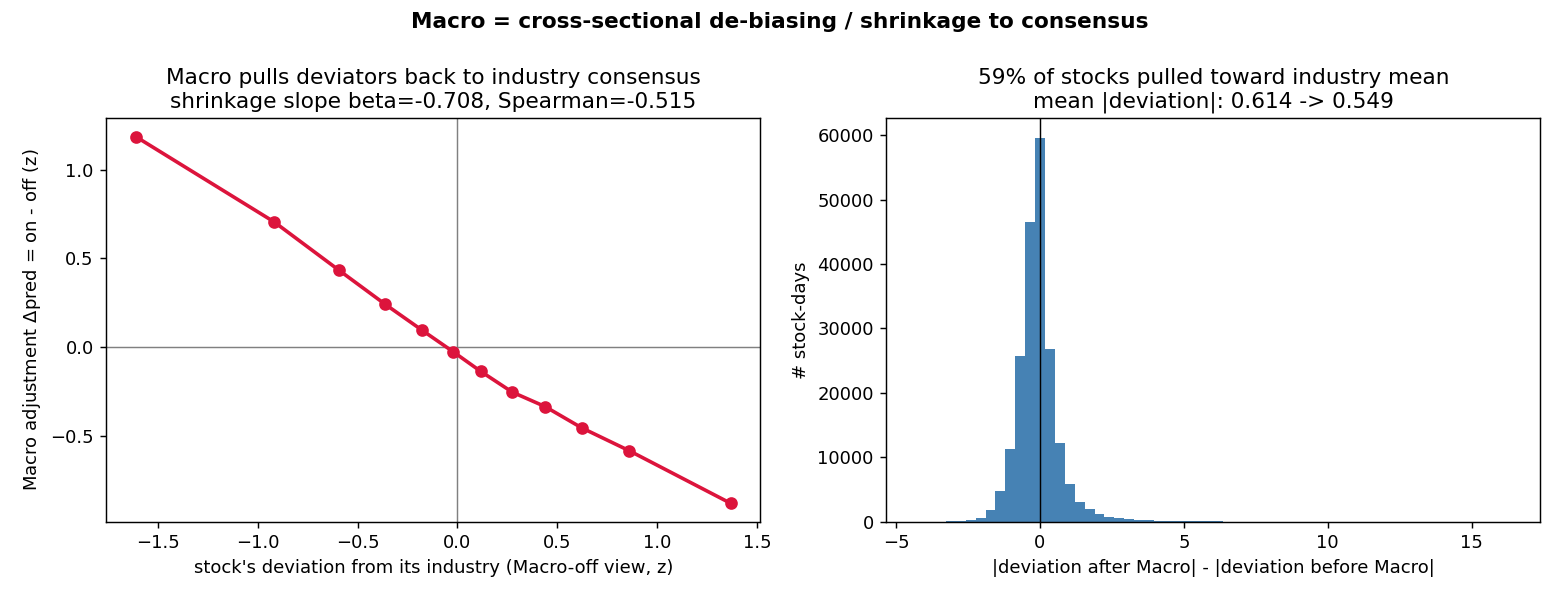
\includegraphics[width=\linewidth]{figures/macro_shrinkage.png}
\caption{Prediction comparison with Macro on / off (baseline, test period
2025-07 to 2026-05, about 200k ``stock-day'' samples). Left: the horizontal
axis is a stock's deviation from its industry mean (under Macro off), and the
vertical axis is Macro on's adjustment to that prediction,
$\Delta\text{pred}$---the further the deviation, the harder the pullback
(shrinkage slope $\beta=-0.708$, Spearman $\rho=-0.515$). Right: distribution
of whole-market mean absolute deviation; $59\%$ of stocks move closer to their
industry mean under Macro on, and the mean drops from $0.614$ to $0.549$. Both
panels point to the same thing: Macro systematically compresses extreme
predictions toward the group center.}
\label{fig:shrinkage}
\end{figure}

Counterfactual shrinkage cannot reproduce Macro's return
(Fig.~\ref{fig:lambda}, Table~\ref{tab:lambda}): shrinking the Macro-off
prediction toward the industry mean per Eq.~\eqref{eq:lambda}, the peaks of two
seeds ($+130\%$ / $+102\%$) are clearly below their respective base
($+166\%$ / $+129\%$), with no rise-then-fall sweet region. Shrinking toward
the industry mean cannot substitute for Macro, indicating that when adjusting
predictions it does not reference the industry mean.

\begin{figure}[H]
\centering
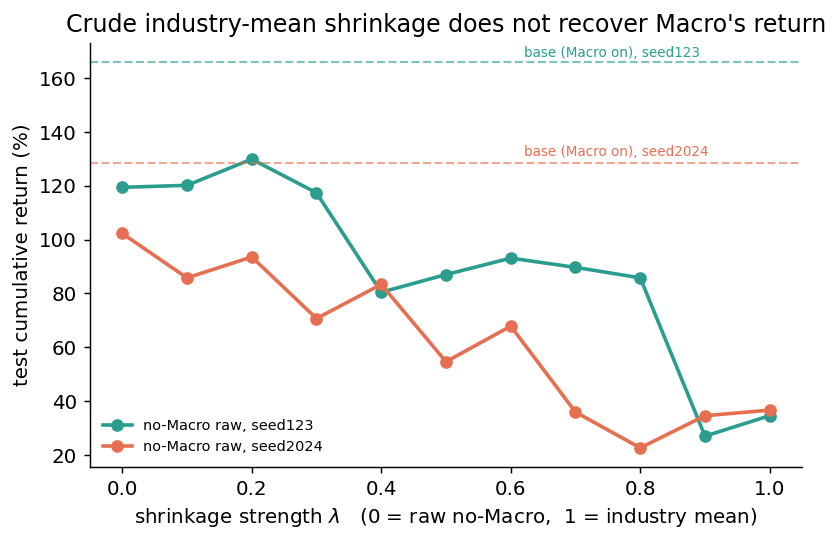
\includegraphics[width=0.66\linewidth]{figures/fig_lambda.png}
\caption{Counterfactual: artificially shrink the Macro-off predictions toward
the industry mean by intensity $\lambda$ ($\lambda{=}0$ no shrinkage,
$\lambda{=}1$ full shrinkage to the industry mean), backtest per $\lambda$, and
see whether ``hand-made de-biasing'' can reproduce Macro's return. The two
solid lines are the test cumulative return of seeds 123 / 2024; the dashed
lines are their respective base (Macro on). At every $\lambda$ the solid lines
are below the dashed lines and there is no rise-then-fall sweet region---
shrinking toward the industry mean cannot substitute for Macro.}
\label{fig:lambda}
\end{figure}

\begin{table}[H]
\centering
\caption{Representative values of the counterfactual (test-period cumulative
return, \%). $\lambda$ is the artificial shrinkage intensity toward the
industry mean ($0{=}$ no shrinkage, i.e., the original Macro-off prediction;
$1{=}$ full shrinkage to the industry mean); the rightmost column ``base'' is
the true return with Macro on. The peaks of the two seeds ($129.9$ at
$\lambda{=}0.2$, $102.3$ at $\lambda{=}0$) are clearly below base ($166.0$,
$128.6$), and the overall trend declines as $\lambda$ grows---using the
industry mean as a substitute cannot reproduce Macro's return.}
\label{tab:lambda}
\begin{tabular}{lccccc}
\toprule
& $\lambda{=}0$ & $\lambda{=}0.2$ & $\lambda{=}0.5$ & $\lambda{=}1$ & base (Macro on) \\
\midrule
seed123  & $+119.4$ & $+129.9$ & $+87.0$ & $+34.6$ & $+166.0$ \\
seed2024 & $+102.3$ & $+93.6$  & $+54.6$ & $+36.7$ & $+128.6$ \\
\bottomrule
\end{tabular}
\end{table}

The true reference lies in the attention distribution. The three Macro layers'
soft grouping has normalized mutual information (NMI---an information-theoretic
measure of how much two groupings overlap; $0$ is no relation, $1$ is full
overlap) with Shenwan industry labels of only $0.22\!\sim\!0.24$---far short of
recovering industries (which would require close to $1$); the attention itself
is high-entropy and diffuse, with each stock on average covering $877$ of the
$\sim$985 stocks on the day, Gini about $0.23$, not a sparse graph along
industry labels; aggregating attention by industry tells the same story
(Fig.~\ref{fig:indagg})---the average attention within the same industry
(diagonal) is even slightly lower than across industries (off-diagonal) (ratio
$0.93$); what really lights up is a few ``hub industry'' columns attended to by
the whole market---a broad, cross-industry graph, not an industry-block
diagonal. Does it then anchor on ``co-movement''? The co-direction rate gives
the whole-market answer, concentrated in \emph{the first layer}: in the first
Macro layer, the same-day co-direction rate of each query stock's top-$10$
focus targets is $61.7\%$, $+3.6$pp above the same-day baseline of ``randomly
picking $10$ stocks'' at $58.1\%$ (aggregated over $208$ trading days, standard
error only $0.4$pp, about $9\times$ the standard error, statistically very
stable but mild in magnitude), and the excess concentrates in the most heavily
attended targets (Fig.~\ref{fig:codir}). The deeper two layers are no longer
above random (in fact slightly lower by $3\!\sim\!4$pp)---deeper-layer
attention acts on representations already refined by earlier layers and no
longer directly anchors the original same-day up/down. So ``connecting by
co-movement structure'' is mainly a first-layer behavior: on each trading day
it dynamically links the query stock to a few partners that \emph{tend} to move
in the same direction that day---a \emph{mild but stable} co-movement tilt
($+3.6$pp, statistically robust but small in magnitude), not a strong relation
graph.

\begin{figure}[htbp]
\centering
\begin{minipage}[b]{0.42\linewidth}\centering
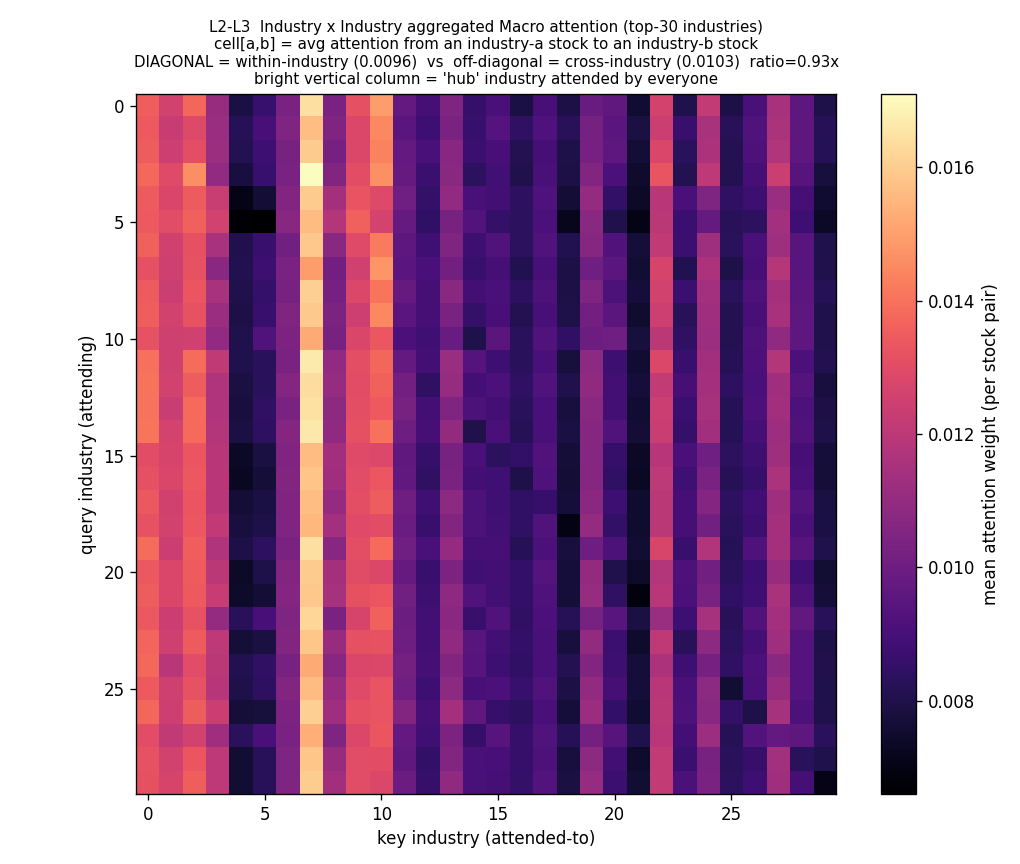
\includegraphics[width=\linewidth]{figures/macro_indagg.png}\\[3pt]
{\small (a) Attention aggregated by industry}
\end{minipage}\hfill
\begin{minipage}[b]{0.54\linewidth}\centering
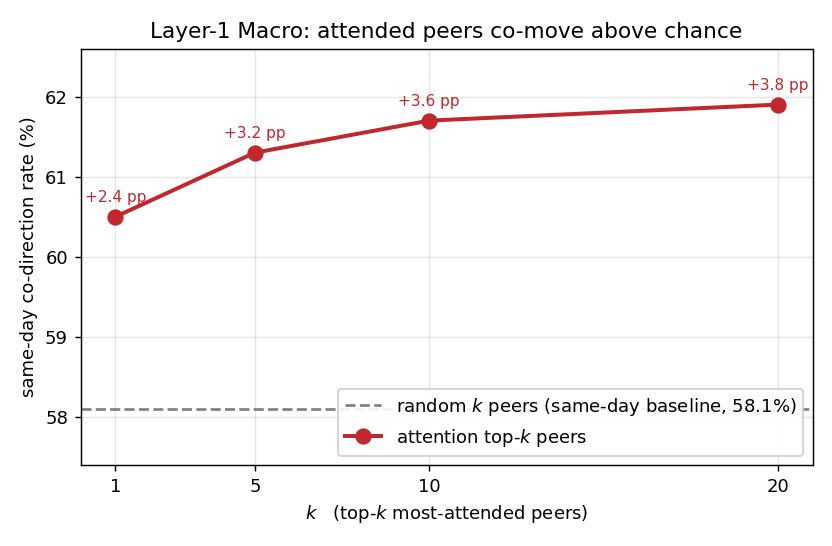
\includegraphics[width=\linewidth]{figures/macro_codir.png}\\[3pt]
{\small (b) Co-movement co-direction rate}
\end{minipage}
\caption{What is the ``pool'' Macro shrinks toward. \textbf{(a)} Attention
aggregated by Shenwan industry (top 30 industries; color is the average
attention ``from a stock in industry-$a$ to a stock in industry-$b$''):
diagonal (same industry) averages $0.0096$, slightly \emph{lower} than
off-diagonal (cross-industry) $0.0103$, ratio $0.93$---no ``same-industry
mutual attention'' block-diagonal; what lights up is a few ``hub industry''
columns attended to by the whole market, a broad, cross-industry graph.
\textbf{(b)} Same-day up/down co-direction rate of the first-layer Macro's
top-$k$ focus targets (all $208$ test days, whole market per day), always about
$+2.4\!\sim\!3.8$pp above the same-day ``randomly pick $k$ stocks'' baseline of
$58.1\%$---more biased toward partners that move in the same direction on the
day, but the excess is mild.}
\label{fig:indagg}
\label{fig:codir}
\end{figure}

The case study corroborates ``non-industry'' from another angle: the
highest-weight focus targets are mostly stocks \emph{across} Shenwan industries
but with real theme / supply-chain links (Fig.~\ref{fig:casestudy}). The
tech-sector 宏发's focus cluster is a cross-industry AI-hardware chain
(optical chip 源杰 $\to$ optical device 天孚 $\to$ optical module Zhongji
中际旭创 / 新易盛, plus PCB 胜宏 / 生益, and power-side 思源 /
金盘); the non-ferrous 神火股份's focus cluster is an electrolytic-aluminum
peer group (天山铝业, 宏桥, 云铝, 中孚, plus copper Jiangxi
Copper). Item-by-item verification is in Appendix~\ref{sec:casestudy-rel}.

\begin{figure}[H]
\centering
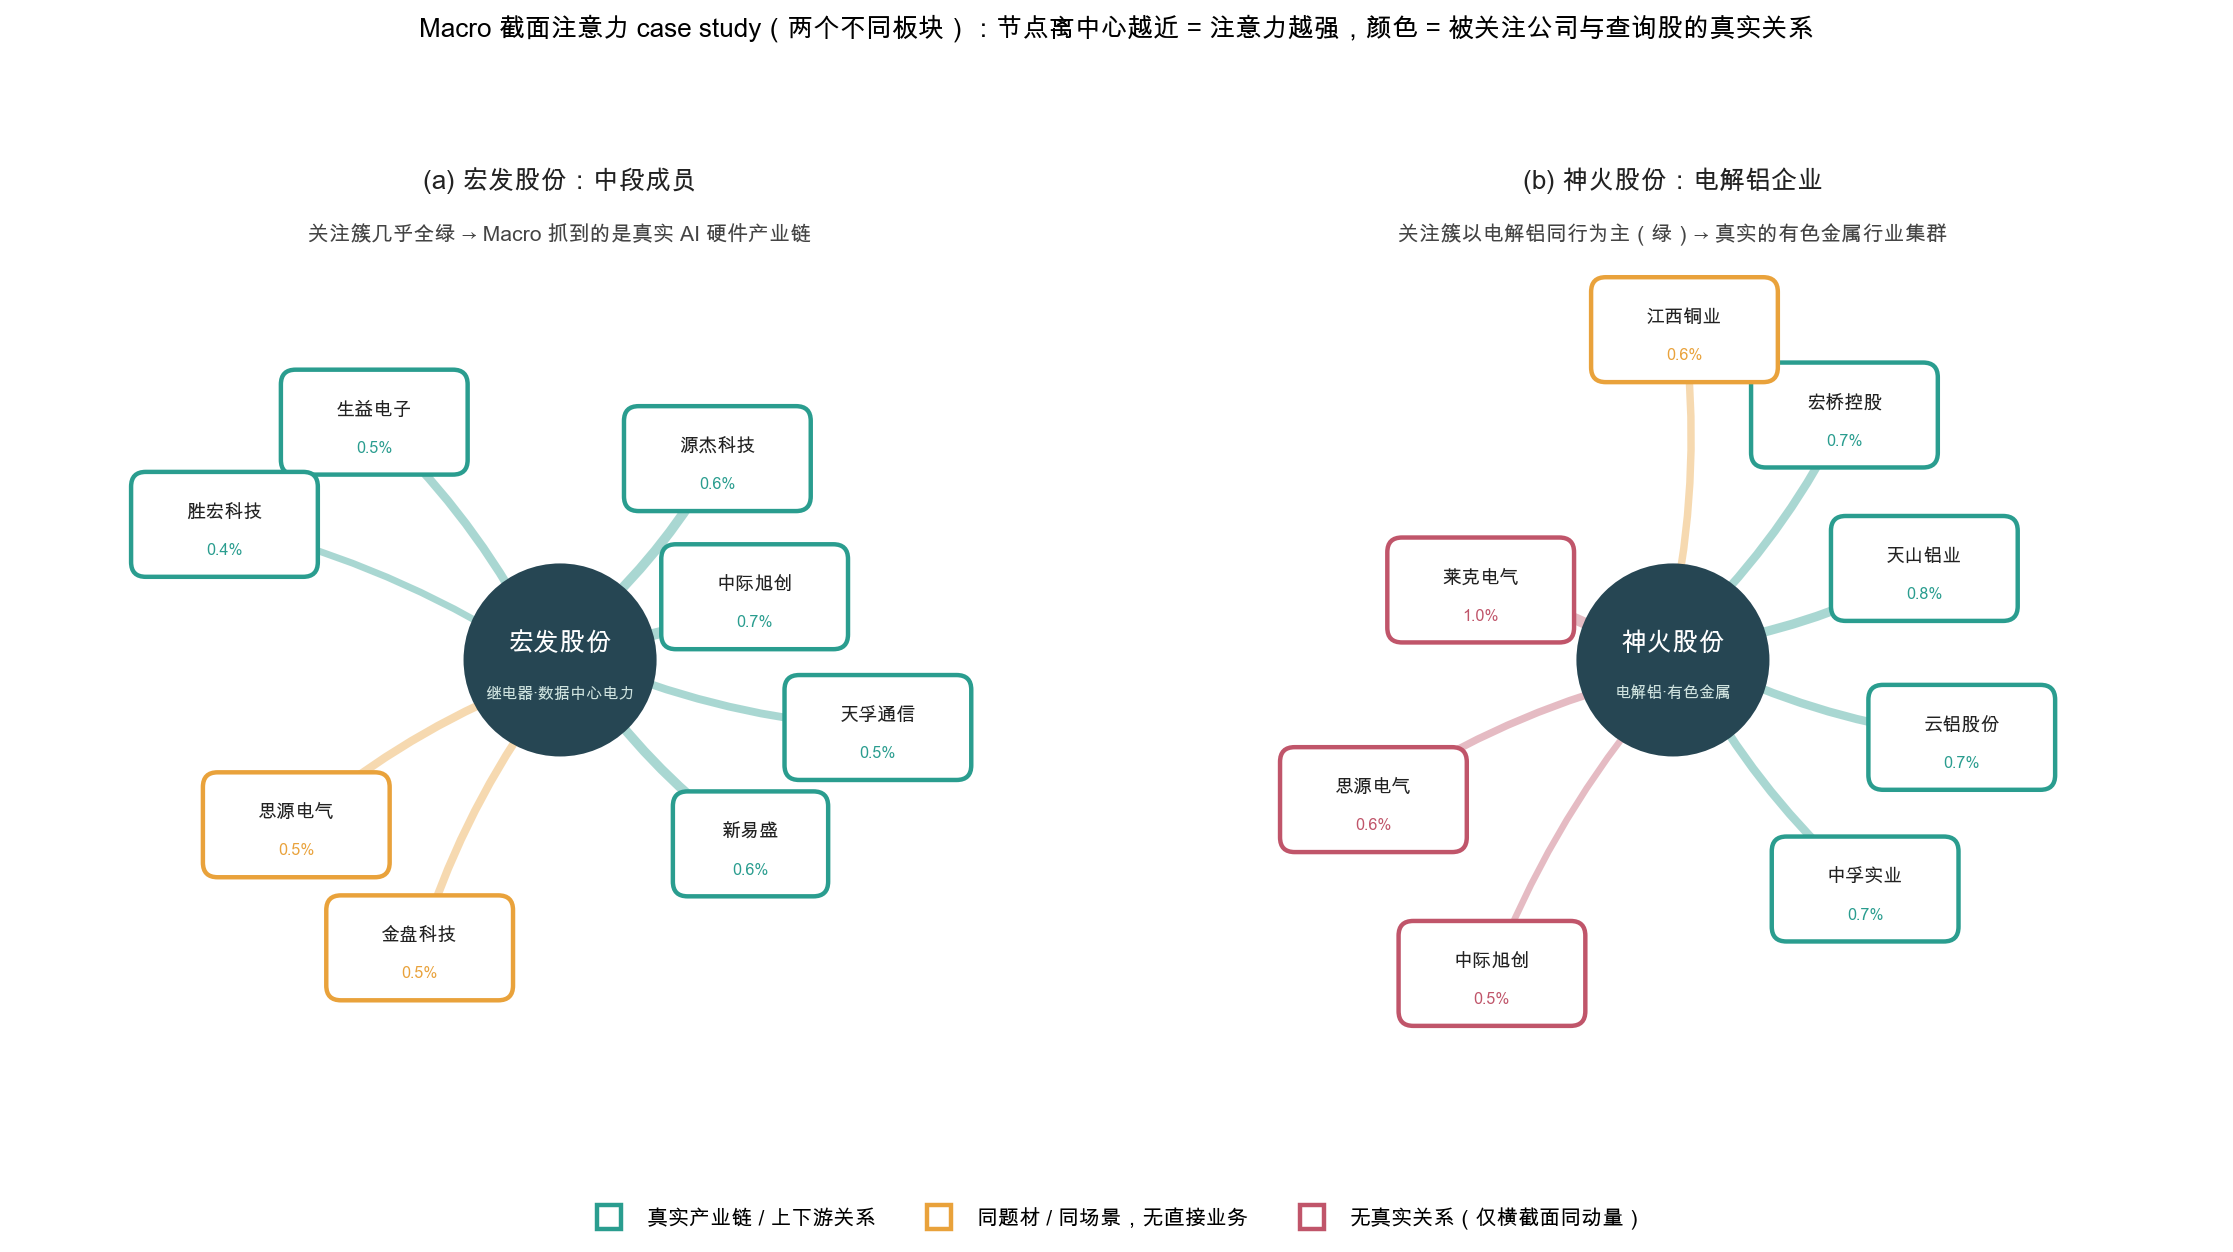
\includegraphics[width=0.96\linewidth]{figures/macro_casestudy.png}
\caption{Visualization of Macro cross-sectional attention (baseline, trading
day 2025-12-11). Each sub-figure is one query stock (center node) and its
highest-weight focus targets: node distance to the center encodes attention
strength; color marks the \emph{real} relation of the focused company to the
query stock (green $=$ real supply chain / same industry, orange $=$ same theme
/ same scenario but no direct business link, red $=$ no real relation, only
cross-sectional co-momentum). (a) 宏发 (tech sector, relays): strong focus
falls on a \emph{cross}-industry real AI-hardware chain (optical chip 源杰
$\to$ optical device 天孚 $\to$ optical module 中际旭创 / 新易盛,
plus PCB 胜宏 / 生益, power-side 思源 / 金盘). (b) 神火股份
(non-ferrous sector, electrolytic aluminum): strong focus locks on a
\emph{same}-industry cluster (天山铝业, 宏桥, 云铝, 中孚, plus
copper 江西铜业). The two cases come from different sectors and have
different relation shapes, but in both the strong focus targets are real
co-rise/co-fall peers---Macro groups by cross-sectional co-movement structure,
not by industry labels (the few red ones are co-momentum noise, e.g.\
莱克电气).}
\label{fig:casestudy}
\end{figure}

\textbf{Analysis.} The four measurements piece together and jointly
point to the same \emph{currently most self-consistent} mechanistic
explanation: Macro is like a learned cross-sectional denoiser. It pulls each
stock's score toward a peer consensus (the de-biasing in
Fig.~\ref{fig:shrinkage}); this consensus is not a static industry
mean---manually shrinking toward the industry mean cannot reproduce its return
(Fig.~\ref{fig:lambda}), the attention grouping's NMI with industry is only
$0.23$, and industry-aggregated attention is even slightly cross-industry
(Fig.~\ref{fig:indagg}); and the peers it shrinks toward do carry
\emph{co-movement structure} on the day---the first-layer focus targets'
co-direction rate is significantly above random (Fig.~\ref{fig:codir}), and the
cross-industry strong focuses in the case study match human-verified theme /
supply-chain links (Fig.~\ref{fig:casestudy}). It must be emphasized:
Fig.~\ref{fig:codir} shows that focused peers have \emph{same-day co-movement
structure} (focus targets are not random), and does \emph{not} prove these
peers carry genuine alpha---``whether borrowing peers to denoise actually buys
a more stable ranking'' is corroborated by the $-46$pp of Macro-off in the
dual-axis ablation (\S\ref{sec:pillars}), not by the co-direction rate itself.

Why this translates into return, the landing point is still noise. Under low
SNR, single-stock score variance is large and individual signals are
unreliable; pulling each stock's estimate toward a pool of correlated peers
averages out specific noise, and \emph{by the James--Stein / empirical-Bayes
framework the variance should decrease}---this is the framework-level
expectation of ``trading a little bias for a lot of variance'' (to reiterate:
this paper does not directly measure the variance drop; \S\ref{sec:macro}'s
theory section already states this; here it is a framework inference, not a
measurement), and it is most worthwhile exactly when noise is largest. This
framework also self-consistently explains two things that otherwise look like
``flaws'': why the attention is so diffuse (each stock on average covers
$877/985$) and why the co-movement is only a mild $+3.6$pp---under this
framework, a good denoising pool should \emph{spread broadly} (broader spread
should reduce variance more) and carry only a \emph{mild} correlation tilt
(enough to suppress the bias of unrelated stocks). Diffuse plus weak
co-movement is not ``failed to find structure''; it is closer to what a
denoiser with a reasonable bias--variance tradeoff should look like.

One more point worth making: no line of supervision tells Macro to find stocks
that rise and fall together; the training objective contains only
cross-sectional ranking. ``Focusing on partners that move with you on the day''
is something the model \emph{learns spontaneously}---because borrowing
correlated peers to denoise lets the ranking be more stable. Co-movement is the
\emph{means}; ranking accuracy is the \emph{end}; this means was not explicitly
specified but emerged on its own under low SNR. Compared with approaches like
RSR or hypergraphs that must be fed an external stock-relation graph, here the
relation graph is formed by the model itself from same-day co-movement (and
weakly so); deeper layers then continue to process representations refined by
earlier layers.

This characterization also has its boundaries. The causal chain of ``denoising
helps'' is, at present, the most self-consistent explanation pointed to by
several lines of evidence; we have not directly measured ``how much the
variance actually dropped and that the return comes exactly from there''; the
co-movement signal itself is not strong and is clear only in the first layer;
for the most extreme momentum leaders (such as 新易盛 with $+424\%$ over the
year), the focus cluster degenerates into ``a plate of strong-trend names
across themes,'' and the model also struggles to distinguish real industry
trends from short-term concept hype (such as 联美控股, which renamed
itself to chase the quantum concept).

% ================================================================ 7 Discussion
\section{Discussion and Limitations}\label{sec:discuss}
\textbf{Checkpoint selection and variance are an under-rated
first-order problem.} The most transferable lesson of this paper is that under
low-SNR cross-sectional selection, ``how to train and select checkpoints''
matters more for the final return than ``which architecture to use.'' The
inverse relation between validation IC and out-of-sample return
(\S\ref{sec:select}) and the $-3\%$ to $+117\%$ swing of the same configuration
across seeds both show that ``improvements'' reported from a single run likely
fall inside the noise band. This requires the evaluation protocol itself to do
the work---best ckpt measures the capability ceiling, validation-selected
measures deployability, multi-seed measures stability, and none is dispensable.

\textbf{Best-ckpt is an upper bound, not a deployable value.} This paper
uses best ckpt as a ``capability ceiling'' to strip off selection variance, but
it picks by test return and is an oracle upper bound; what is actually
deployable is the validation-selected checkpoint. The report gives both to avoid
misreading the upper bound as live performance. How to select checkpoints
robustly without peeking at the test set (multi-checkpoint ensembling, or
stability criteria beyond validation IC) is a direction worth pursuing.

\textbf{The ceiling of common-mode market information.} The
cross-sectional ranking objective largely cancels \emph{common-mode} market
signals that affect all stocks similarly: when all stocks are pushed in the
same direction by the same market move, their relative order barely changes,
and what we optimize and evaluate is the relative order. Therefore
\emph{common-mode} market information has a naturally limited incremental value
for cross-sectional alpha---this is why this paper uses only a few market
indices by default and does not rely on elaborate market-modulation structures.
\textbf{Must be distinguished from Macro:} what has ``limited
incremental value'' here is the \emph{common mode} (market-wide common mode,
the part canceled by cross-sectional ranking), whereas Macro's pillar status
(turning it off costs $-46$pp, \S\ref{sec:pillars}/\ref{sec:macro}) relies
\emph{not} on the common mode but on \emph{the relative structure between
individual stocks}---pulling each stock toward a peer consensus and removing
stock-specific noise. The common mode is the canceled background; relative
structure is the signal Macro feeds on; the two are not contradictory.

\textbf{The method is more robust than the return number.} Under the
unified protocol, \msqa{} returns higher than all reproduced baselines, but the
return number is not the point of this paper---it depends on seed and selection
and swings widely under the variance redline. What stands is the method: each
axis can be turned off independently, so the pillar role can be directly
verified (\S\ref{sec:pillars}); attention weights can be hooked out, so whom
Macro attends to can be attributed (\S\ref{sec:macro}); every conclusion is
pressed under the $\pm60$pp redline, so genuine effects and noise can be
told apart.

\textbf{Limitations.} (i) The test window is short, financial data is
noisy, and the statistical confidence of absolute returns is limited;
(ii) training uses CSI 300 and backtest uses top1000, so the two protocols are
not fully consistent; (iii) some configurations (especially some seeds) save
sparse checkpoints, so the best ckpt is ``best among existing checkpoints''
rather than the continuous optimum; (iv) no news / sentiment external text data
is used---such information partly acts on prices as sentiment or events, is
related to the ``ceiling of common-mode market information'' above, and is
often already laggy when made public; our features use only price-volume $+$
fundamentals $+$ money flow.

% ================================================================ 8 Conclusion
\section{Conclusion}\label{sec:conclusion}
This paper works on A-share cross-sectional selection and proposes
\textbf{two model-design innovations}. First, the dual-axis interaction
(time-axis Micro $+$ cross-section-axis Macro) is reorganized into a decoupled,
stackable, per-axis-disableable feature-extraction primitive, the \msq{} Block,
whose multi-layer stacking lets the two axes iteratively re-read each other.
Second, the $(S,T,D)$ representation is kept throughout, causal temporal
attention is used, and dense cross-sectional ranking supervision is applied at
every time step. Under the unified evaluation protocol (best ckpt $+$ multi-seed
$+$ variance redline), the robust conclusions that survive the redline can be
summarized as \textbf{three findings}. \emph{(1) Both designs are ablatively
confirmed effective}: removing either dual axis costs significant return (error
bars do not overlap with base), stacking brings visible iterative gains, and
dense supervision also significantly outperforms last-step-only (error bars do
not overlap under either protocol, \S\ref{sec:abl-dense}). \emph{(2) The most
self-consistent mechanistic explanation of Macro is a cross-sectional
denoiser}: it pulls each stock's prediction toward the consensus of a
data-driven set of correlated peers and suppresses single-stock noise (the soft
grouping's NMI with Shenwan industries is only $0.23$, so it is neither the
industry mean nor an external relation graph), and low SNR is exactly the
precondition for this denoising to be effective---but this is the most
self-consistent \emph{explanation} under current evidence, not a causal proof.
\emph{(3) Validation IC is inversely related to out-of-sample return}; the
standard selection criterion systematically picks worse-generalizing models,
underscoring the necessity of the evaluation protocol.

The judgment running through the paper is: under low SNR, how you train and
select checkpoints is more decisive of success or failure than how the
architecture looks. \msqa{} returns higher than all reproduced baselines, but
its real foothold is the method---the dual axes can be turned off per-axis to
locate pillars, attention can be hooked out for attribution, and every
conclusion is pressed under the $\pm60$pp redline to tell true from false.
Future work can proceed along the limitations: (1) robust checkpoint selection
without peeking at the test set (targeting the selection failure); (2)
re-examining absolute returns over a longer test window and a unified
train / backtest universe (targeting limitations i/ii); (3) using a
time-pooling control to additionally measure the contribution of ``retaining
the time dimension'' itself, i.e.\ the \emph{representation design} half not
covered by the dense-supervision ablation (\S\ref{sec:abl-dense}); (4) directly
measuring the prediction-variance reduction brought by Macro to push denoising
from ``most self-consistent explanation'' to causal verification; (5) a
definitive equal-parameter ``wide single layer vs.\ stacking'' comparison, and
feeding interpretability conclusions back into architecture improvements for
re-verification.

% ================================================================ Highlights
\section*{Experimental Highlights}
\begin{itemize}
  \item The dual-axis interaction is made into a per-axis-disableable \msq{}
        Block---each axis can be removed and re-measured independently, so the
        pillar role can be directly falsified rather than resting on narrative.
  \item An evaluation protocol that separates genuine effects from noise: best
        ckpt measures the capability ceiling, validation-select measures
        deployability, multi-seed pins down variance, and a $\pm60$pp redline
        tells true from false. This is the project's most transferable output.
  \item A falsifiable, and currently most self-consistent mechanistic
        explanation for Macro---it \emph{behaves like} a learned cross-sectional
        denoiser: NMI only $0.23$, the $\lambda$ sweep rules out the industry
        mean as a substitute, ruling out ``the anchor is industry''; the
        whole-market co-movement test measures that first-layer focus targets
        do carry same-day co-movement structure (mild but significant; note
        this is co-movement, not genuine alpha). But no direct causal evidence
        of variance reduction has been measured, so this is an
        \emph{explanation} rather than a proof; interpretability does not stop
        at narrative.
  \item Two counter-intuitive findings: validation IC is inversely related to
        out-of-sample return ($-0.75$); holding the model signal fixed and
        changing only the trading strategy can move the return by $130$pp, the
        same order as architectural changes.
\end{itemize}

% ================================================================ Appendix
\appendix

This appendix gives the input features, ablations, and diagnostic details not
expanded in the main text, under the same protocols (best ckpt, multi-seed
seeds 42/123/2024, $\pm60$pp redline). Reading them together has a unified
meaning: the returns reported in the main text do not depend on some carefully
tuned hyperparameter. Apart from a few designs that trigger collapse (binary
labels, an overly short time window, simultaneously removing causal and
Gaussian), the multi-seed returns of changes such as head count, sub-layer
order, neighbor bandwidth, sparsification, and turnover regularization all fall
within base's ($+155\pm19$) redline band and are indistinguishable from noise.
See the summary in Table~\ref{tab:appendix}.

\section{Input features: 35 price-volume / fundamental / money-flow factors}\label{sec:features}
All features are computed along each stock's own time series
(\texttt{groupby(ts\_code)}, never across stocks), uniformly prefixed with
\texttt{f\_}, and are not globally standardized---that is left to subsequent
rolling standardization to prevent leakage. The baseline uses 35 factors in 7
groups (Table~\ref{tab:features}): the price-volume technical group (the first
five sub-groups, 27 factors) is a subset of Qlib's Alpha158 factor
library~\cite{qlib}; the 6 fundamentals are taken directly from Tushare
\texttt{daily\_basic}; the 2 money-flow factors are self-constructed (full
formulas below). Larger factor sets (\texttt{medium}$\approx 80$,
\texttt{full}$\approx 158$, the latter a fuller Alpha158 subset) are used for
factor-count scaling experiments.

\begin{table}[H]
\centering\small
\caption{The 35 factors of the baseline input (\texttt{feature\_set=basic}).
Source tags: A $=$ Alpha158 subset~\cite{qlib}, D $=$ Tushare
\texttt{daily\_basic}, S $=$ self-constructed. $O/H/L/C/V$ are
open / high / low / close / volume, $r_1=C_t/C_{t-1}-1$,
$\mathrm{MA}_k/\mathrm{VMA}_k$ are $k$-day means, and $\mathrm{std}_k$ is the
$k$-day rolling standard deviation.}
\label{tab:features}
\begin{tabular}{@{}p{1.9cm}p{6.0cm}cp{3.4cm}@{}}
\toprule
Group (source) & Factor & Count & Definition \\
\midrule
Multi-scale momentum (A) & \texttt{f\_ret\_k}, $k\in\{1,2,3,5,10,20,30,60\}$ & 8 & $C_t/C_{t-k}-1$ \\
MA deviation (A) & \texttt{f\_close\_ma\_k}, $k\in\{5,10,20,30,60\}$ & 5 & $C_t/\mathrm{MA}_k-1$ \\
Volatility (A) & \texttt{f\_vol\_k}, $k\in\{5,10,20,30,60\}$ & 5 & $\mathrm{std}_k(r_1)$ \\
Candlestick (A) & \texttt{f\_kmid}, \texttt{f\_klen}, \texttt{f\_kup}, \texttt{f\_klow} & 4 & see below \\
Volume (A) & \texttt{f\_vol\_ratio\_k} $(k{\in}\{5,10,20\})$; \texttt{f\_vol\_chg\_1}; \texttt{f\_amount\_chg\_1} & 5 & $V_t/\mathrm{VMA}_k$; 1-day change of volume / amount \\
Fundamentals (D) & \texttt{f\_turnover\_rate}, \texttt{f\_turnover\_rate\_f}, \texttt{f\_volume\_ratio}, \texttt{f\_pe\_ttm}, \texttt{f\_pb}, \texttt{f\_ps\_ttm} & 6 & turnover / free-float turnover / volume ratio / PE / PB / PS (fields used directly) \\
Money flow (S) & \texttt{f\_mf\_net\_ratio}, \texttt{f\_mf\_big\_small\_diff} & 2 & see below \\
\midrule
\multicolumn{2}{@{}l}{Total} & 35 & \\
\bottomrule
\end{tabular}
\end{table}

\noindent\textbf{Candlestick pattern (following Alpha158's definition).}
Let open / high / low / close be $O,H,L,C$:
\[
\texttt{f\_kmid}=\frac{C-O}{O},\quad \texttt{f\_klen}=\frac{H-L}{O},\quad
\texttt{f\_kup}=\frac{H-\max(O,C)}{O},\quad \texttt{f\_klow}=\frac{\min(O,C)-L}{O}.
\]

\noindent\textbf{Self-constructed money-flow factors (full formulas).}
Let $A$ be the day's turnover amount (in thousands of CNY), $M$ the day's net
money inflow (in ten-thousand CNY, Tushare \texttt{net\_mf\_amount}), and
$B_{lg},B_{elg},B_{sm}$ the buy amounts of large / extra-large / small orders
(in ten-thousand CNY):
\begin{align*}
\text{\texttt{f\_mf\_net\_ratio}} &= \mathrm{clip}\!\Big(\frac{M\times 10^{4}}{A\times 10^{3}},\ -5,\ 5\Big)
= \mathrm{clip}\!\big(10M/A,\,-5,\,5\big),\\[3pt]
\text{\texttt{f\_mf\_big\_small\_diff}} &= \frac{(B_{lg}+B_{elg})-B_{sm}}{(B_{lg}+B_{elg})+B_{sm}+1}.
\end{align*}
These two are the only non-Alpha158 factors in the baseline 35, added
specifically to give A-shares a \emph{money-flow} dimension beyond price and
volume---A-shares are retail-dominated and prices are often pushed by money
flow and sentiment (\S\ref{sec:intro}); Tushare's \texttt{moneyflow} provides
exactly the money-structure information Alpha158 lacks. We explain each below.

\textbf{(1) \texttt{f\_mf\_net\_ratio}: net-inflow intensity.} The day's
\emph{net inflow} divided by the \emph{turnover amount} (after unifying units to
CNY, clipped to $[-5,5]$; the conversion factor $10$ comes from Tushare quoting
turnover in thousands and money flow in ten-thousands). It measures ``what
fraction of today's turnover in this stock is driven by net buying'': $>0$
means net inflow (buy-side dominant, possibly accumulation), $<0$ means net
outflow. The reason for \emph{dividing by turnover amount} rather than using
the absolute net inflow directly is that stocks differ in turnover scale by
orders of magnitude, so absolute amounts are not cross-sectionally comparable;
after normalization to a ratio, this ``money-flow strength'' signal can be used
to rank stocks cross-sectionally within the same day---fitting the
cross-sectional selection goal of this paper. The $[-5,5]$ clip suppresses
extreme values from suspension-resumption and one-day anomalies.

\textbf{(2) \texttt{f\_mf\_big\_small\_diff}: main-force vs.\ retail
buy structure.} $(\text{large}+\text{extra-large buy})-\text{small buy}$
divided by the sum of the three (the $+1$ in the denominator prevents
divide-by-zero), normalized into $[-1,1]$. In A-shares, large / extra-large
orders usually correspond to institutions or hot-money (the ``main force''),
and small orders to retail, so this factor characterizes \emph{who is buying}:
$>0$ means main-force buying is stronger than retail (main force entering),
$<0$ means retail is taking the other side and the main force may be
distributing. In a retail-dominated, sentiment-driven market, ``who is buying''
is often more informative than ``how much was bought''---stocks with net
main-force buying have a higher probability of subsequent relative strength;
this is exactly a cross-sectionally comparable signal added from the
\emph{structural} dimension of money flow, beyond price, volume, and valuation.

\section{Architecture ablations}\label{sec:abl-arch}
This group checks whether the main-text return depends on a particular value of
some architectural hyperparameter. We change each in turn and backtest; the
following all fall within base's ($+155\pm19$) redline band, except the last
one.

\textbf{Attention head count.} Head count determines how many relation
patterns the model can track in parallel and is the most-tuned hyperparameter.
Changing Micro (time axis) heads from the default $4$ to $2$ / $8$ gives
$+186\pm37$ / $+163\pm27$; changing Macro (cross-section) heads from the
default $2$ to $1$ / $4$ gives $+161\pm26$ / $+165\pm33$. All four overlap with
base; the return is insensitive to head count.

\textbf{Sub-layer order.} Each Block is by default Micro-then-Macro.
Reversing to cross-section-then-time gives $+142\pm20$, overlapping with
base---which axis goes first does not change the result, because after
multi-layer stacking the two alternate anyway.

\textbf{Sparse Macro.} Cross-sectional attention by default connects the
whole market. If each stock attends only to its top-$30$-scoring neighbors, the
return is $+161$ (two seeds, same order as base), no
worse than full connection. This is consistent with \S\ref{sec:macro}: what
Macro needs is a few stable consensus anchors; the dense long-tail connections
are dispensable noise.

\textbf{Multi-scale Micro.} Letting different stacked layers use
different lookback lengths ($8/5/3$ days bottom-up) to cover multiple time
scales gives $+162\pm30$, overlapping with single-scale base---multi-scale
brings no extra return.

\textbf{Width.} Widening the representation dimension $D$
($64/128/256$, best-ckpt, three seeds): $+79\pm19\%$ / $+155\pm19\%$ /
$+154\pm17\%$. $D{=}64\to128$ catches up to the base level, but
$128\to256$---doubling parameters again---stays flat ($155\to154$, within the
error bar): widening saturates at base's width. This contrasts sharply with
stacking depth ($L{:}3\to4\to5$ keeps rising from $155$ to $187$, $201$): the
same extra parameters help in depth but not in width, corroborating that the
depth gain comes from iterative re-reading rather than pure capacity
(see \S\ref{sec:depth}).

\textbf{Removing causal / global attention.} The items above are all
``changing it does no harm''; this one is the counterexample. Simultaneously
removing Micro's causal mask (switching to bidirectional) and the Gaussian
prior degenerates time-axis attention into unconstrained global attention,
giving $+52$ (\emph{single seed seed42}). Per our decision rule this must be
read carefully: a single seed is not enough to pin down the exact value, but
its drop relative to base ($+155$) is about $103$pp, nearly twice the
$\pm60$pp redline and far beyond seed-noise magnitude, so the
\emph{direction} that ``letting everything go significantly worsens results''
should be robust (the exact magnitude and multi-seed confirmation are left to
future work). This shows that the temporal inductive bias of ``looking only at
the past, with a neighbor preference'' is genuinely valuable, and it is one of
the few negatively directed changes with a stable direction.

\subsection{Micro's recency prior: Gaussian bandwidth and time window}\label{sec:abl-micro}
Micro adds a Gaussian prior decaying with time distance on top of the
time-axis self-attention (\S\ref{sec:m-block}), controlled by two knobs; we
ablate each. \textbf{Gaussian bandwidth $\sigma$} controls how strongly
``neighbor preference'' is enforced: $\sigma{=}2/4/8$ gives $+139$ / $155$ /
$+112$ respectively, all overlapping with base; the bandwidth is insensitive.
\textbf{Removing the Gaussian prior entirely} gives $+169\pm34$ (three
seeds), also within the noise band---whether this prior is added makes
\emph{no significant difference}; it behaves more like a harmless inductive
bias than a source of return. \textbf{Time window $\tau$} (how many days
back each time step can see at most) has a clear lower bound: $\tau{=}1$
(looking only at the previous day) collapses to $+33\pm14$, while $\tau\ge3$
returns to the same order as base ($\tau{=}3/5/8/15$ about
$+135/+134/+155/+152$). So Micro does rely on neighbor weighting, but as long
as the window is not too short the exact length is insensitive.

\section{Training and regularization}\label{sec:abl-train}
Additional training-side experiments---adversarial training (FGSM perturbation
$\varepsilon{=}0.1$, $+181\pm14$) and turnover regularization (penalizing
turnover in the training objective, $\lambda{=}0.1$, $+139\pm72$)---do not
stably cross the variance redline; both have multi-seed returns within base's
redline band as well. The systematic comparison of training objectives
themselves (regression / ranking / classification) is in \S\ref{sec:objective}.

\begin{table}[H]
\centering
\caption{Appendix ablation summary (test cumulative return, best-ckpt,
multi-seed). Base $=+155\pm19$; unless noted, seeds 123/2024.}
\label{tab:appendix}
\begin{tabular}{lcc}
\toprule
Ablation & Return (mean$\pm$std) & Reading \\
\midrule
Micro heads ($2$ / $8$, default $4$)   & $+186$ / $+163$ & overlaps base \\
Macro heads ($1$ / $4$, default $2$)   & $+161$ / $+165$ & overlaps base \\
Sub-layer order (Macro before Micro)       & $+142\pm20$    & overlaps base \\
Sparse Macro (per stock attend top-$30$)  & $+161$         & no worse than full \\
Multi-scale Micro (lookback $8/5/3$ days)     & $+162\pm30$    & overlaps base \\
Gaussian bandwidth ($\sigma{=}2/4/8$)        & $+139$ / $155$ / $+112$ & $\sigma$ insensitive \\
Remove Gaussian ($\sigma\to0$, three seeds)      & $+169\pm34$    & overlaps base \\
Time window ($\tau{=}1/3/5/8/15$)       & $+33$/$135$/$134$/$155$/$152$ & $\tau{=}1$ collapses; $\tau\ge3$ same order \\
Adversarial training ($\varepsilon{=}0.1$, three seeds)& $+181\pm14$  & within redline \\
Turnover regularization ($\lambda{=}0.1$, three seeds) & $+139\pm72$    & within redline \\
Remove causal $+$ remove Gaussian (global attention)     & $+52$ (seed42) & below redline (single seed, direction robust) \\
\bottomrule
\end{tabular}
\end{table}

\subsection{Training recipe: learning rate, optimizer, scheduler}\label{sec:abl-recipe}
The previous section (Table~\ref{tab:appendix}) examined the \emph{architecture
and regularization} sidelines under the best-ckpt protocol; here we turn to the
\emph{training recipe} itself---learning rate, optimizer, LR scheduler, and
dropout, and deliberately report under the
\textbf{deployable ``validation-select $\times$ 3 seeds'' protocol}
(\S\ref{sec:select}). The reason: training-recipe changes directly affect
``when convergence happens and which ckpt validation selects,'' so they should
be examined under the very protocol that exposes selection and seed variance,
to see which choices survive the $\pm60$pp noise. The backtest engine in this
table is a simplified TopK portfolio (top1000 universe, open-price execution),
different from the institutional strategy of the main-text tables, so it should
be used only for \emph{within-table relative comparison}.

\begin{table}[H]
\centering
\caption{Training-recipe ablation: test cumulative return, validation-select
$\times$ 3 seeds, simplified TopK backtest engine (top1000 / open-price
execution). The default base $=$ AdamW, lr $10^{-5}$, no scheduler, dropout
$0.1$; the same-protocol reference is $+67\%$ (seed 42). SGD-family learning
rates are scaled up as is customary (momentum / Nesterov $10^{-3}$, Adagrad
$10^{-2}$).}
\label{tab:recipe}
\begin{tabular}{llcl}
\toprule
Knob & Configuration & Return (mean$\pm$std) & Reading \\
\midrule
Learning rate   & $10^{-4}$ (high)       & $+41\pm25$           & \\
         & $5\times10^{-5}$       & $\mathbf{+107\pm48}$ & sweet spot \\
         & $10^{-6}$ (low)       & $+33\pm15$           & \\
\midrule
Optimizer   & SGD$+$Nesterov         & $-5\pm3$    & \\
         & SGD$+$Momentum         & $-1.5\pm3$  & uniformly, stably \\
         & RMSprop                & $+14\pm19$  & worse than AdamW base \\
         & Adagrad                & $+33\pm16$  & \\
\midrule
Scheduler   & $+$cosine              & $+89\pm82$  & \\
         & $+$cosine\,warmup      & $+99\pm82$  & higher mean but \\
         & $+$step                & $+97\pm97$  & drowned in seed noise \\
\midrule
Dropout  & $0$                    & $+35\pm26$  & \\
         & $0.2$                  & $+94\pm55$  & overlaps base \\
\bottomrule
\end{tabular}
\end{table}

Three conclusions. \textbf{(1) The optimizer is the only cross-seed-robust
hard constraint.} Even after scaling up SGD-family learning rates by
$100$--$1000\times$ as is customary (momentum / Nesterov with $10^{-3}$,
Adagrad with $10^{-2}$, vs.\ AdamW's $10^{-5}$), their three-seed returns stay
glued near $0$ (Nesterov $-5\pm3$, SGD$+$Momentum $-1.5\pm3$, variance only
$3$pp), while \emph{all} AdamW-based configurations---base and all learning-rate
/ scheduler / dropout variants---are clearly higher. This is one of the few
genuine conclusions whose variance is far below the redline and that holds on
every seed: sparse, high-noise cross-sectional gradients need adaptive step
sizes. \textbf{(2) The learning rate has a sweet spot.} Within AdamW,
$5\times10^{-5}$ ($+107$) beats $10^{-4}$ ($+41$) and $10^{-6}$ ($+33$); both
too high and too low hurt; base's chosen $10^{-5}$ is slightly conservative.
\textbf{(3) Scheduler and dropout are largely drowned by seed noise.}
The means of the three schedulers ($+89\sim99$) look higher than base, but the
std is as high as $80$--$97$pp---the step scheduler gives a scary $+186\%$ on
seed 42 but $-7\%$ on seed 2024. This is exactly a living sample of the
``selection $\times$ seed'' trap of \S\ref{sec:select}: a single seed is enough
to dress up a pure-noise knob as a ``best practice,'' and three seeds expose it
immediately.

\section{Statistical construction of the Macro diagnostic figures}\label{sec:macro-prov}
For the four Macro diagnostic figures in \S\ref{sec:macro}, how their data are
computed step by step from raw predictions / attention to the final figure
(sample unit, aggregation, statistics, and the definition of the random
baseline) is summarized uniformly in Table~\ref{tab:macro-prov} for
reproducibility and reading; ``construction'' here means the statistical
definition, not the plotting software.

\begin{table}[H]
\centering
\caption{Data construction (provenance) of the Macro diagnostic figures. All
predictions come from the same set of base models (seeds 42/123/2024),
Macro-on / Macro-off inference, test period 2025-07 to 2026-05, backtest
protocol as in \S\ref{sec:setup}.}
\label{tab:macro-prov}
\begin{tabularx}{\linewidth}{l>{\raggedright\arraybackslash}X>{\raggedright\arraybackslash}X}
\toprule
Figure & Sample unit / input & Computation \& statistics \\
\midrule
Fig.~\ref{fig:shrinkage} (shrinkage) & All ``stock-days'' ($\sim$200k); on/off predictions each cross-sectionally $z$-scored per day &
OLS fit of $\Delta\text{pred}{=}\hat r^{\mathrm{on}}{-}\hat r^{\mathrm{off}}$ on ``deviation from industry mean'' (single fit, $\beta$, \emph{not} winsorized, only non-finite values removed) and Spearman $\rho$; industry mean computed from Macro-\emph{off} $z$ values; pullback ratio and mean absolute deviation pooled over stock-days \\
Fig.~\ref{fig:lambda} (counterfactual) & Per-industry (per day $\times$ per industry) mean of Macro-off predictions &
Per $\lambda\in\{0,0.1,\dots,1\}$, shrink toward industry mean per Eq.~\eqref{eq:lambda} and backtest, yielding per-$\lambda$ test cumulative return (result file \texttt{lambda\_shrink.csv}); seeds 123/2024 only (seed42 absent from the result file); compared with Macro-on base \\
Fig.~\ref{fig:indagg} (industry aggregation / NMI) & $A_{\mathrm{off}}$ (last layer, head-averaged, diagonal removed) &
Industry$\times$industry cell $=$ average attention from stocks in industry $a$ to stocks in industry $b$; NMI is the normalized mutual information between the clusters (spectral clustering of the symmetrized $A_{\mathrm{off}}$, $k{=}\min(12,\#\text{industries})$) and Shenwan industry labels; a 200-permutation industry-label permutation test is also run \\
Fig.~\ref{fig:codir} (co-direction) & Per trading day $\times$ per query stock, $A_{\mathrm{off}}$'s top-$k$ focus targets ($k{\in}\{1,5,10,20\}$) &
Co-direction $=$ fraction with the same sign of same-day up/down; random baseline is the analytical same-day expected co-direction $p^2{+}(1{-}p)^2$ (result file column \texttt{rand\_agree}, numerically verified, market-wide up/down already deducted); the ``excess over random'' is \emph{aggregated per trading day} ($n{=}208$) for mean$\pm$SE \\
Fig.~\ref{fig:casestudy} (case examples) & A single day (2025-12-11), top-10 focus targets of two query stocks &
Intuition support only; node colors (real supply chain / same industry / same theme / unrelated) are \emph{manually annotated by the author}, not model outputs; item-by-item verification in \S\ref{sec:casestudy-rel} \\
\bottomrule
\end{tabularx}
\end{table}

\subsection{Verification of the real relations behind Macro's focused stocks}\label{sec:casestudy-rel}
The case study in \S\ref{sec:macro} shows that Macro's highest-weight focus
targets are mostly stocks across Shenwan industries but plausibly of the same
theme. To verify whether these cross-industry focuses correspond to
\emph{real} supply-chain / theme links, we manually looked up the public
businesses and concept affiliations of the query stocks and their top focus
companies in Fig.~\ref{fig:casestudy} (trading day 2025-12-11) one by one. The
conclusions can be summarized in four points.

\textbf{(1) 宏发: attention reconstructs a real AI-hardware supply
chain.} 宏发 itself is a real participant on the power side of AI data
centers (HVDC high-voltage DC relays for 800V DC architectures). Its top focus
falls almost entirely within the broad AI-hardware supply chain and contains
two verifiable sub-chains (Table~\ref{tab:casestudy}): (1) the optical
communication chain---源杰 (optical chip) $\to$ 天孚 (optical device) $\to$
中际旭创 / 新易盛 (optical module), where 中际旭创 early
on incubated 源杰 to secure optical-chip supply; (2) AI-server PCB---
胜宏 (Nvidia GB200/GB300 PCB Tier-1 supplier) and 生益
(high-speed-switch PCB). Plus same-theme targets on the data-center power side
(思源, 金盘). This is a cluster spanning $4$ Shenwan industries but
genuinely existing in the supply chain.

\begin{table}[H]
\centering
\caption{Verification of the real relations among 宏发's top focus companies
(excerpt, verified online).}
\label{tab:casestudy}
\begin{tabular}{lll}
\toprule
Focused company & Business & Real relation to 宏发 / each other \\
\midrule
源杰科技 & Optical chip & Top of the optical-communication chain; supplies 中际旭创 / 新易盛 \\
天孚通信 & Optical device & Core component supplier for 中际旭创 / 新易盛 optical modules \\
中际旭创 & Optical module & Global \#1 optical-module market share; early incubator of 源杰 \\
新易盛   & Optical module & Optical-module leader; with 中际旭创 / 天孚 nicknamed the ``易中天'' trio \\
胜宏科技 & GPU-board PCB & Nvidia GB200/GB300 PCB Tier-1 \\
生益电子 & Switch PCB & Main supplier of 800G high-speed-switch PCB \\
思源电气 / 金盘科技 & Power transmission / Transformer & Data-center power side, same scenario as 宏发 \\
\bottomrule
\end{tabular}
\end{table}

\textbf{(2) 神火股份: a same-industry electrolytic-aluminum cluster.} The
same ``catching real relations'' also holds in the \emph{non-ferrous} sector,
but manifests as a \emph{same}-industry cluster rather than a cross-industry
supply chain. Among the top focus targets of the electrolytic-aluminum company
神火股份, 天山铝业, 宏桥, 云铝, and 中孚 are all
electrolytic-aluminum peers, plus copper leader 江西铜业, forming a real
non-ferrous-metal / electrolytic-aluminum industry cluster (only the top-ranked
莱克电气 is an unrelated home-appliance momentum stock). It and
宏发 belong to the non-ferrous and tech sectors respectively and have
different relation shapes (same-industry cluster vs.\ cross-industry supply
chain), jointly showing that the ``peers'' Macro catches are real economic
links rather than noise.

\textbf{(3) Extreme momentum leaders: attention degenerates into a
``strong-trend plate across themes''.} The contrast appears on the most extreme
momentum names. The top focus of optical-module leader 新易盛 (up $+424\%$
in 2025, the AI-compute champion) contains \emph{no} other optical-module or
optical-chip stock; instead it is all lithium (中矿资源, 盛新锂能), oil shipping (招商轮船), Hainan free-trade-port sealing (海峡股份, Hainan
Rubber)---leaders in \emph{completely different tracks but with similarly
extreme momentum}; the focus basket of AI-PCB leader 胜宏 is likewise
dominated by resource themes such as lithium / tungsten / civil explosives /
heating. So the clustering axis is \emph{cross-sectional momentum strength}
rather than the supply chain---when the query stock is a mid-chain member of a
supply chain (宏发), the chain is reconstructed exactly; when it is an
extreme-momentum outlier, attention degenerates into a cross-theme plate.

\textbf{(4) Hub stocks $=$ market-sentiment bellwethers.} 中矿资源,
阳光电源, 广东宏大, 招商轮船, and 联美控股 recur across multiple
query stocks; they belong to $5$ unrelated Shenwan industries but are all
2025 high-momentum leaders in their respective tracks---corroborating that
Macro treats ``the day's strongest trend names'' as repeatedly referenced
consensus anchors. 联美控股 deserves a warning: its main business is
heating, and it only rose four consecutive limit-ups because of renaming to
``联美量子'' and investing in 摩尔线程, riding AI / quantum
concept hype (the renaming, investment, and consecutive limit-ups are all in
public market records)---showing that Macro \emph{cannot distinguish} a real
industry trend from short-term concept hype, which is a blind spot of this
interpretability method and echoes the boundary discussion in
\S\ref{sec:macro}.

% ================================================================ Appendix B Trading strategy
\section{Impact of the trading strategy on return}\label{sec:strategy}
The model outputs a cross-sectional ranking \emph{signal}; turning it into real
return requires another layer of portfolio construction: how many names to
hold, how to weight them, whether to cap industry concentration. A
quantitative-investment survey~\cite{survey} points out that trading /
portfolio strategy is a key step from an alpha signal to final return. To
quantify the impact of this step, we \emph{fix} one set of predictions (base
best ckpt, corresponding to $+170.9\%$ in Table~\ref{tab:main}), change only
the trading strategy, and re-run the backtest (other protocols as in
\S\ref{sec:setup}).

Results are in Table~\ref{tab:strategy} and Fig.~\ref{fig:strategy}: the final
return of the \emph{same signal} swings between $+95\%$ and $+225\%$, a span of
$130$pp---larger than the effect of the overwhelming majority of architectural
changes in the main text. \emph{Position concentration} is the strongest
lever: holding only the top $5$ names gives $+225\%$ (Sharpe $3.34$), declining
monotonically to $+95\%$ when holding $30$; relaxing the industry-concentration
cap also raises return (no cap $+195\%$ vs.\ base's $20\%$ cap $+171\%$); and
equal-weight vs.\ score-weighted makes almost no difference ($+170.9\%$ vs.\
$+171.3\%$). The trading strategy is not an appendage after the model; its
impact on return is the same order as architectural changes. But concentrated
holdings amplify stock-specific risk while raising return---our test window is
short, so drawdown indicators may underestimate the tail risk of concentrated
strategies; the main-text main results uniformly use the more robust
configuration of $10$ holdings with a $20\%$ industry cap, a compromise between
return and robustness rather than the return optimum.

\begin{figure}[H]
\centering
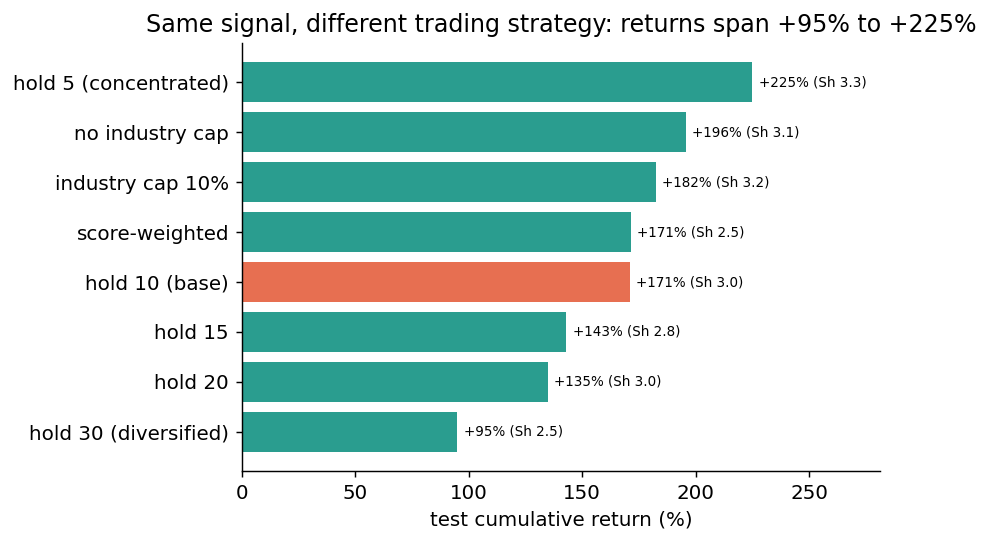
\includegraphics[width=0.82\linewidth]{figures/fig_strategy.png}
\caption{Impact of the trading strategy on return (fixed base predictions).
The same signal's return ranges from $+95\%$ to $+225\%$ under different
portfolio constructions; the more concentrated the holdings, the higher the
return (and the more stock-dependent); base (orange) takes the compromise of
$10$ holdings. Sharpe values are in parentheses.}
\label{fig:strategy}
\end{figure}

\begin{table}[H]
\centering
\caption{Impact of the trading strategy on return (fixed base best-ckpt
predictions, test period).}
\label{tab:strategy}
\begin{tabular}{lcccc}
\toprule
Strategy & Cumulative return & Sharpe & Max drawdown & Turnover \\
\midrule
Hold 5 (concentrated)    & $+225.0\%$ & $3.34$ & $-16.0\%$ & $0.29$ \\
Hold 10 (base)   & $+170.9\%$ & $2.99$ & $-14.7\%$ & $0.30$ \\
Hold 15           & $+143.0\%$ & $2.78$ & $-12.7\%$ & $0.31$ \\
Hold 20           & $+134.7\%$ & $2.96$ & $-11.3\%$ & $0.31$ \\
Hold 30 (diversified)   & $+94.9\%$  & $2.53$ & $-12.4\%$ & $0.32$ \\
Score-weighted (hold 10)  & $+171.3\%$ & $2.53$ & $-17.2\%$ & $0.60$ \\
No industry cap           & $+195.5\%$ & $3.10$ & $-14.7\%$ & $0.31$ \\
Industry cap $10\%$      & $+182.3\%$ & $3.19$ & $-13.0\%$ & $0.31$ \\
\bottomrule
\end{tabular}
\end{table}

For the open-source release, we further re-test the report-backed depth
versions under the more concentrated $n=5$, $20\%$ industry cap,
sell-only-when-dropping-out-of-top-200 protocol. This supplementary sweep uses
the research top1000 universe, open-price execution, and fee protocol, so it
should not be directly equated to the public M-0-M baseline display; its role
is to show the model ability of deeper M\textsuperscript{2} Blocks under the
complete-factor research panel. Results are in
Table~\ref{tab:release-strategy-sweep}: M2.2/L5, released publicly as M-2-M,
reaches $+354.59\%$ under the high-concentration strategy and is the main
research highlight. M2.1/L4 remains ablation and depth-comparison evidence
rather than a public main line. The public \path{scripts/benchmark_research.py}
runner also reproduces the main setting on a compatible top1000 research
panel, with M-2-M at $+354.34\%$, Sharpe
$3.99$, and max drawdown $-17.68\%$.

\begin{table}[H]
\centering
\caption{Supplementary strategy sweep for the public models (top1000 /
open-price execution / fees included; predictions fixed, only portfolio rules
changed).}
\label{tab:release-strategy-sweep}
\begin{tabular}{lccccc}
\toprule
Model & $n=5$, cap20 & $n=10$ base & $n=30$, cap20 & $n=10$, no cap & $n=10$, cap10 \\
\midrule
M2.1 / L4 seed42 ep17   & $+147.21\%$ & $+224.12\%$ & $+107.46\%$ & $+215.79\%$ & $+172.03\%$ \\
M2.2 / L5 seed2024 ep20 & $\mathbf{+354.59\%}$ & $+235.33\%$ & $+113.26\%$ & $+253.00\%$ & $+196.96\%$ \\
\bottomrule
\end{tabular}
\end{table}


\section{Code and reproduction notes}\label{sec:repro}
The public entry points for training / inference / benchmark reproduction are
as follows. Full historical experiments require an external data panel; the
static site, checkpoint inference path, and baseline smoke path are directly
reproducible.
\begin{itemize}
  \item \textbf{Website data rebuild.} Compatibility entry point is
  \path{build/update_daily.py}; it calls \path{build/update_research_live.py}
  to rebuild the M-1-M/M-2-M historical curves in \path{docs/data/data.json}
  from a compatible research panel.
  \item \textbf{Checkpoint inference.} Entry point is
  \path{build/inference.py}, which regenerates predictions for the public
  research-curve checkpoints M-1-M and M-2-M; single-model tests should write
  to a temporary path to avoid overwriting committed caches.
  \item \textbf{Research benchmark.} Entry point is
  \path{scripts/benchmark_research.py}, which reproduces the research backtest
  protocol on a compatible historical top1000 panel and industry file; this
  path is the public benchmark basis.
  \item \textbf{Baseline training.} The public training entry is
  \path{scripts/train_baseline.py} with \path{configs/baseline.json}. The
  repository provides a smoke test on the committed cache; full baseline
  training requires passing in a historical panel compatible with
  \path{docs/DATA_SCHEMA.md}.
  \item \textbf{Data contract.} The full research data is not released
  with the repository; the public repository provides the BaoStock + AKShare +
  efinance public-data adapter, the field schema, and the baseline code path. To reproduce the
  experimental tables you need to prepare your own A-share daily panel for
  2017--2026 with matching fields.
  \item \textbf{Research-table boundary.} The multi-seed, ablation,
  interpretability, and strategy-sweep tables in this report are frozen
  research records. The public repository guarantees that the method, model
  structure, benchmark runner, and baseline reproduction path are auditable;
  re-running the full historical research tables depends on external data and
  compute.
  \item \textbf{Environment and randomness.} Python~3.9+ and PyTorch are
  recommended. Randomness is controlled by seeds (\texttt{torch.manual\_seed} /
  \texttt{cuda.manual\_seed\_all}), but bit-level determinism is not promised;
  research results should therefore be read under the multi-seed statistical
  protocol rather than relying on a single run.
\end{itemize}



% ================================================================ References
\begin{thebibliography}{99}
\small
\bibitem{lstm} S.~Hochreiter and J.~Schmidhuber. Long Short-Term Memory. \emph{Neural Computation}, 9(8):1735--1780, 1997.
\bibitem{alstm} Y.~Qin, D.~Song, H.~Cheng, W.~Cheng, G.~Jiang, and G.~W.~Cottrell. A Dual-Stage Attention-Based Recurrent Neural Network for Time Series Prediction. \emph{IJCAI}, 2017.
\bibitem{sfm} L.~Zhang, C.~Aggarwal, and G.-J.~Qi. Stock Price Prediction via Discovering Multi-Frequency Trading Patterns. \emph{KDD}, 2017.
\bibitem{transformer} A.~Vaswani et al. Attention Is All You Need. \emph{NeurIPS}, 2017.
\bibitem{rsr} F.~Feng, X.~He, X.~Wang, C.~Luo, Y.~Liu, and T.-S.~Chua. Temporal Relational Ranking for Stock Prediction. \emph{ACM Transactions on Information Systems (TOIS)}, 37(2):1--30, 2019.
\bibitem{advalstm} F.~Feng, H.~Chen, X.~He, J.~Ding, M.~Sun, and T.-S.~Chua. Enhancing Stock Movement Prediction with Adversarial Training. \emph{IJCAI}, 2019.
\bibitem{dtml} J.~Yoo, Y.~Soun, Y.-c.~Park, and U.~Kang. Accurate Multivariate Stock Movement Prediction via Data-Axis Transformer with Multi-Level Contexts. \emph{KDD}, 2021.
\bibitem{tra} H.~Lin, D.~Zhou, W.~Liu, and J.~Bian. Learning Multiple Stock Trading Patterns with Temporal Routing Adaptor and Optimal Transport. \emph{KDD}, 2021.
\bibitem{hist} W.~Xu, W.~Liu, L.~Wang, Y.~Xia, J.~Bian, J.~Yin, and T.-Y.~Liu. HIST: A Graph-based Framework for Stock Trend Forecasting via Mining Concept-Oriented Shared Information. \emph{arXiv:2110.13716}, 2021.
\bibitem{crossformer} Y.~Zhang and J.~Yan. Crossformer: Transformer Utilizing Cross-Dimension Dependency for Multivariate Time Series Forecasting. \emph{ICLR}, 2023.
\bibitem{stockmixer} J.~Fan and Y.~Shen. StockMixer: A Simple yet Strong MLP-based Architecture for Stock Price Forecasting. \emph{AAAI}, 2024.
\bibitem{master} T.~Li, Z.~Liu, Y.~Shen, X.~Wang, H.~Chen, and S.~Xiong. MASTER: Market-Guided Stock Transformer for Stock Price Forecasting. \emph{AAAI}, 2024.
\bibitem{gausstransformer} Q.~Ding, S.~Wu, H.~Sun, J.~Guo, and J.~Guo. Hierarchical Multi-Scale Gaussian Transformer for Stock Movement Prediction. \emph{IJCAI}, 2020.
\bibitem{survey} L.~Cao, et al. From Deep Learning to LLMs: A Survey of AI in Quantitative Investment. \emph{arXiv:2503.21422}, 2025.
\bibitem{qlib} X.~Yang, W.~Liu, D.~Zhou, J.~Bian, and T.-Y.~Liu. Qlib: An AI-oriented Quantitative Investment Platform. \emph{arXiv:2009.11189}, 2020. (Source of the Alpha158 factor library, \texttt{microsoft/qlib}.)
\end{thebibliography}

\end{document}
